\documentclass{article}
\usepackage[utf8]{inputenc}
\usepackage{amsfonts}
\usepackage{geometry}
\usepackage{amsmath}
\usepackage{todonotes}
\usepackage{amsthm}
\usepackage{hyperref}
\usepackage{physics}
\usepackage{graphicx}
\usepackage{subcaption}
% \usepackage[square,sort,comma,numbers]{natbib}

\newtheorem{theorem}{Theorem}

\newcommand{\ob}[1]{\textcolor{blue}{\bf [[[Ollie: #1]]]}}
\newcommand{\mce}[1]{\textcolor{purple}{[Matt: #1]}}
\newcommand{\pmr}[1]{\textcolor{purple}{[Patricio: #1]}}
\newcommand{\avi}[1]{\textcolor{red}{[Avi: #1]}}

\geometry{a4paper, top=1cm, bottom=3cm, left=1.5cm, right=3.5cm,heightrounded,bindingoffset=5mm }

\title{Wavelets}
\author{ Q.~Baghi, O.~Burke, G.~Mentasti, A.~Vajpeyi}
\date{May 12, 2023}

\begin{document}

\maketitle

\tableofcontents


\section{Introduction}
Gravitational wave detector noise exhibits non-stationarity due to transient fluctuations, long-term spectral drifts, and data-stream gaps. 
These effects induce correlations across frequency samples, exacerbating the challenges of frequency domain analysis. 
One method to address this is to use a time-frequency data analysis approach, employing discrete wavelet wavepackets. 
Mapping time domain data onto a uniform grid of time-frequency pixels mitigates correlations, particularly for locally stationary noise. 
In this work, we introduce an open-source GPU-accelerated Python library for gravitational wave time-frequency data analysis, PyWavelet. 
We provide a suite of examples, demonstrating Bayesian analysis of GW signals using the time-frequency domain versus traditional methods, while accounting for non-stationary noise effects. Detailed mathematical derivations for the wavelet domain analysis are available in supplementary materials.


\section{Definitions}
We are given a data stream in time domain, consisting of a set of N samples of a \textbf{real} quantity  s at times $\{t_k\}_{k=0\dots N-1}$ in a total time of observation $T$
\begin{align}\label{st_definition}
x[k]=x(t_k)\qquad,\qquad k=\{0\dots N-1\}\;,
\end{align}
and all of the information we have lies in these N points. We define the time sampling rate and the Nyquist frequency as
\begin{align}
r_s&\equiv\frac{1}{\Delta t}\equiv\frac{N}{T}\;,\nonumber\\
f_{\rm max}&=\frac 1 2r_s\;,\nonumber\\
\Delta f \equiv 1/(2\Delta t)
\end{align}
With that respect, if we set $t_0=0$, we can write $t_k=k\delta t$. In the frequency domain (please note that we are not going to use the following expression, but I am writing it for sake of clarity) we know that the data stream $\{x_k\}$ can be discrete-Fourier-trasformed to a set of other N \textbf{complex} numbers\footnote{One can show that there is not more information that the original data: even if it seems that now we have 2N real numbers, one than needs to go back to the time domain eventually to recover physical quantities.}
\begin{align}
x^{\rm Fourier}[j]=\sum_{k=0}^{N-1}x[k] e^{-\frac{2\pi i}{N}jk}\;,
\end{align}
where $j=0\dots N-1$. If we wanted to represent $x^{\rm Fourier}$ as a function of some frequencies, we would have $x^{\rm Fourier}[j]=x^{\rm Fourier}(f_j)$ where $f_j=j\frac{f_{max}}{N}$.
\subsection{The wavevelet domain}\label{sec:wavelet_domain}
The wavelet domain considers a transformation of \eqref{st_definition} that takes the original N points and reshape them into a $N_t\times N_f$ grid, where then
\begin{align}\label{NtNf_def}
N=N_t\,N_f\;,
\end{align}
must hold. The underlying idea, is to chunk the data stream into $N_t$ chunks and to perform a frequency analysis of each one of those. Please note that N is fixed, but $N_t$ is an arbitrary choice you can make. The only constraint is obviously $1\le N_t\le N$. Consequently, the constraint applies for $N_f$: $1\le N_f\le N$.
Given that choice we can define
\begin{align}\label{DTDF}
\Delta T&\equiv\frac{T}{N_t}\;,\nonumber\\
\Delta F&\equiv\frac{f_{\rm max}}{N_f}=\dots=\frac{1}{2\Delta T}\;.
\end{align}
The last expression shows how the Nyquist theorem still holds. Once you fix $N_t$ (or equivalently $N_f$, $\Delta T$ or $\Delta F$) the grid is uniquely identified.
With these definitions, we can introduce the wavelet decomposition of our data stream:
\begin{align}
\label{eq:inverse_wavelet_decomposition}
x[k]=\sum_{n=0}^{N_t-1}\sum_{m=0}^{N_f-1}w_{nm}g_{nm}[k]\;,
\end{align}
where $g_{nm}[k]$ are the wavelet basis elements. Notice here that in the limit as $N_{f}\rightarrow N$ the series above \eqref{eq:inverse_wavelet_decomposition} approaches as Fourier series. To be concrete, if $N_{f} \rightarrow N$, then $N_{t}\rightarrow 1$ since $N = N_{t}N_{f}$ and, from the definition of the (inverse) discrete fourier transform, observe that 
\begin{align}
h(t_{k}) &= \sum_{m = 0}^{N -1}\tilde{h}(f_{m})e^{2\pi i f_{m}t_{k}} = \sum_{m = 0}^{N - 1}\omega_{0m}g_{0m}[k]\, ,\nonumber
\end{align}
modulo factors of $N$. Hence, for the Fourier series, we identify $g_{0m}[k] = \exp(2\pi i f_{m}t_{k})$ as the Fourier basis elements and $\omega_{0m} = \tilde{h}(f_{m})$ as the Fourier coefficients. We can show that they can be always chosen to be (quasi-)orthonormal, i.e.
\begin{align}
\label{eq:orthonormality}
\sum_{k=0}^{N-1}g_{nm}[k]g_{pq}[k]=\delta_{np}\delta_{mq}\;,
\end{align}
allowing us to rewrite our problem to the search of the coefficients
\begin{align}\label{wnm_def}
w_{nm}=\sum_{k=0}^{N-1}x[k]g_{nm}[k]\;.
\end{align}
The problem now translates to find a set of good basis elements $g_{nm}[k]$ and, given those elements, the set of coefficients $w_{nm}$ for any arbitrary data stream $x[k]$.
\subsection{The wavelet basis}
To do so, we need to define firstly the Meyer window functions in the frequency domain $\phi(\omega)$
\begin{align}
\label{eq:meyer_window_freq}
\tilde\phi(\omega)=\left\{\begin{array}{lr}
\frac{1}{\sqrt{\Delta \Omega}} & |\omega|<A \\
\frac{1}{\sqrt{\Delta \Omega}} \cos \left[\nu_d\left(\frac{\pi}{2} \frac{|\omega|-A}{B}\right)\right] &A \leq|\omega| \leq A+B
\end{array}\right.\;,
\end{align}
whose plot is in figure \ref{fig:phi_omega} and where $\nu_d(x)$ is the normalized incomplete Beta function
\begin{align}
\nu_d(x)=\frac{\int_0^x y^{d-1}(1-y)^{d-1} d y}{\int_0^1 y^{d-1}(1-y)^{d-1} d y}\;.
\end{align}
%
\begin{figure}[ht!]
\centerline{
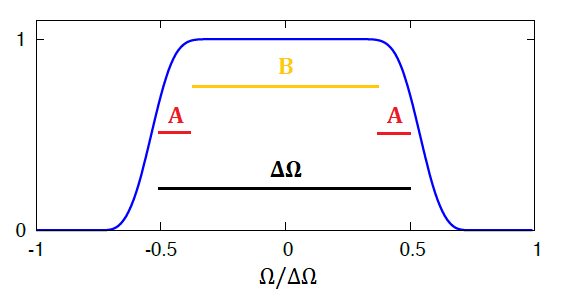
\includegraphics[width=0.6\textwidth,angle=0]{figures/phi_omega.png}
}
\caption{The window function for the WDM wavelets for the choice $d = 4$, $A =\Delta\Omega/4$ and $B = \Delta\Omega/2$. For this choice of window parameters the wavelets are better localized in frequency than they are in time. Here the overall normalization
is arbitrary.}
\label{fig:phi_omega}
\end{figure}
%
The free parameters to be chosen are $A$ and $d$, while all the others are defined consequently:
\begin{align}
\label{eq:window_bandwidth}
\Delta\Omega&=2\pi\Delta F\nonumber\\
B&=\Delta\Omega-2A
\end{align}
Next step, since the Meyer window function is built in the frequency domain, we can define the wavelet basis in the frequency domain
\begin{align}
\label{eq:gnm}
\tilde g_{mn}(\omega)=e^{-in\omega\Delta T}\left(C_{nm}\tilde\phi(\omega-m\Delta\Omega)+C^*_{nm}\tilde\phi(\omega+m\Delta\Omega)\right)
\end{align}
where $C_{nm}=1$ for $(n + m)$ even and $C_{nm}=i$ for $(n + m)$ odd.
(\textcolor{red}{Very unclear now how these coefficients})
From this point, there are two ways to compute the coefficients $w_{nm}$ of \eqref{wnm_def}, a slow one and a faster one.
\subsubsection{The slow method: $w_{nm}$ directly from the data stream}
\begin{itemize}
    \item We first of all anti-Fourier transform (\textcolor{red}{Please note that also this time, in both Cornish and Necula papers there's not a precise definition in terms of formulae for this passage}) the function $\tilde \phi(\omega)\to\phi(t)$.
    \item We cut the function $\phi(t)$ in the range $|t|<q\Delta T$ with $q$ another arbitrary quantity (Cornish set it to $q=16$ to produce the plots).
    \item For the discrete time samples of $s[k]$ we compute the weights
    \begin{align}
    \label{eq:direct}
w_{n m}=\sqrt{2} \Delta t \Re \left[C_{n m} \sum_{k=-K / 2}^{K / 2-1} e^{i \pi k m / N_f} x\left[n N_f+k\right] \phi[k]\right]\;,
\end{align}
where $K=2qN_f$
\end{itemize}
\subsubsection{The faster method: passing through $x_m[n]$ first}
\begin{itemize}
    \item We produce the discrete Fourier transform of the data stream $x[k]\to X[l]$
    \item We compute the "windowed-Fourier transforms"
    \begin{align}
    \label{eq:wdft}
        x_m[n]=\sum_{l=-N_t/2}^{N_t/2-1}e^{-2\pi iln/N_t}X[l+mN_t/2]\tilde\phi[l]
    \end{align}
    where we remind that the index $m$ runs over the frequency coordinates in the grid defined in \eqref{NtNf_def}, while $n$ runs over the time ones.
    \item We compute the weights
    \begin{align}
    \label{eq:fast}
        w_{nm}=\sqrt{2}(-1)^{nm}\Re\left[C_{nm}x_m[n]\right]
    \end{align}
    \item \textbf{As an alternative}, accordingly to Cornish, the objects $x_m[n]$ "can be computed using a
    FFT of length $N_t$ for each $m$". \textcolor{red}{Again, the statement is cryptic and not supported by formulas. Necula did not mention even mention this method with the last formulas I have just written.} This alternative to the method is supposed to speed up the algorithm a lot (the total cost of the WDM transform would be less than twice the cost of the full FFT in this case).
\end{itemize}


\section{Statistics of wavelet coefficients}

\subsection{With stationary noise}

In this section, we assume that the time series $x[k]$ is a realization of the stationary, zero-mean Gaussian noise of one-sided power spectral density (PSD) $S(f)$. We wish to derive the approximate covariance of the wavelet coefficients $w_{nm}$. We start from Eqs.~\eqref{eq:wdft} and \eqref{eq:fast} and compute the covariance of two wavelet coefficients. Let us define the complex quantity $\underbar{w}_{nm}$ the same way as $w_{nm}$ in Eq.~\eqref{eq:fast} but without the real part operator. We have
\begin{align}
\label{eq:covariance_1}
    \operatorname{E}\left[\underbar{w}_{nm} \underbar{w}_{n'm'}^{\ast}\right] = 2 C_{n m}  C_{n' m'}^{\ast} \sum_{l=-N_t / 2}^{N_t / 2-1} \sum_{l'=-N_t / 2}^{N_t / 2-1}   e^{-2 i \pi (ln  - l' n' )/ N_t} \operatorname{E}\left[ X\left[l + m N_t / 2 \right] X\left[l' + m' N_t / 2 \right]^{\ast}  \right] \tilde{\phi}[l] \tilde{\phi}[l']^{\ast}
\end{align}
Using the circulant approximation of the stationary time series covariance, we have
\begin{align}
    \operatorname{E}\left[X[k]X[k]^{\ast}\right] \approx \delta_{k k'} \frac{N}{2 \Delta t}S(f_k),
\end{align}
where $f_k = k / T$. The prefactor comes from the fact that we assumed no special normalization of the discrete Fourier transform $X$, that is 
\begin{equation}
    X[l] = \sum_{k=-N/2}^{N/2-1} x[k] e^{-2\pi i k l / N} 
\end{equation}
Therefore, the expectation term in Eq.~\eqref{eq:covariance_1} is non-zero only when 
\begin{align}
\label{eq:lconditions}
    l + m N_t / 2 & = l' + m' N_t / 2 \text{ or} \nonumber \\
    l + m N_t / 2 & = N_t - l' - m' N_t / 2.
\end{align}
The index $l' = l^{\prime}_0 = l + (m-m') N_t / 2$ verifies the first equality in Eqs.\eqref{eq:lconditions}. There are only two non-zero terms in the sum over $l'$ corresponding to $l^{\prime}_0$ and $N_t - l^{\prime}_0$. Eq.~\eqref{eq:covariance_1}  becomes
\begin{align}
\label{eq:covariance_2}
    \operatorname{E}\left[\underbar{w}_{nm} \underbar{w}_{n'm'}^{\ast}\right] & \approx 2 C_{n m}  C_{n' m'}^{\ast} \sum_{l=-N_t / 2}^{N_t / 2-1}   e^{-2 i \pi (ln  - (l + (m-m')N_t/2 )n' )/ N_t} \frac{N}{2 \Delta t}S\left( f_{l + m N_t / 2} \right)  \nonumber \\
    & \times \tilde{\phi}[l] \left(\tilde{\phi}[l + (m-m') N_t / 2]^{\ast} + \tilde{\phi}[-l + (2 - m + m') N_t / 2]^{\ast} \right)
\end{align}

From Eq.~\eqref{eq:meyer_window_freq} we see that the Meyer window function $\tilde\phi(\omega)$ is non-zero for angular frequencies such that $|\omega| < \Delta \Omega $. Using Eq.~\eqref{eq:window_bandwidth}, the frequency indices $l$ corresponding to this condition are
\begin{align}
\label{eq:bandwidth-condition}
    \left| \frac{2 \pi l}{T} \right| \leq 2 \pi \Delta F.
\end{align}
Eq.~\eqref{eq:covariance_2} exhibits the product $\tilde{\phi}[l] \tilde{\phi}[l + (m-m') N_t / 2]^{\ast}$. Let us assume that the window is zero outside the bandwith $\Delta \Omega$ (which is approximately true) and equal to $1/\sqrt{\Omega}$ inside. Then the product takes non-zero values only if $l$ and $l + (m-m') N_t / 2$ simultaneously satisfy the condition \eqref{eq:bandwidth-condition}, which is only possible if $m=m'$. The same is true for the second product. As a result, two wavelet frequency bins are approximately uncorrelated.

Furthermore, from the relations in Eq.~\eqref{NtNf_def} and Eq.\eqref{DTDF} we can express $\Delta F = 1 / (2 \Delta t N_f) = N_t / (2 \Delta t N)$ to check that the condition \eqref{eq:bandwidth-condition} is strictly equivalent to $|l| \leq N_t / 2$. Therefore, Eq.~\eqref{eq:covariance_2} becomes
\begin{align}
\label{eq:covariance_3}
    \operatorname{E}\left[\underbar{w}_{nm} \underbar{w}_{n'm'}^{\ast}\right] & \approx \frac{2 N}{\Delta t} \delta_{m m'} C_{n m}  C_{n' m}^{\ast} \sum_{l=-N_t / 2}^{N_t / 2-1}   e^{-2 i \pi l (n-n') / N_t} S\left(f_{l + m N_t / 2}\right)  | \tilde{\phi}[l] |^{2} 
\end{align}
The above expression is a circuclar convolution of the PSD with some kernel 
\begin{align}
    K_{n, n', m}[l] &  \equiv \frac{2 N}{\Delta t} C_{n m}  C_{n' m}^{\ast} | \tilde{\phi}[l] |^{2}  e^{-2 i \pi l (n-n') / N_t}.
\end{align}
If we Taylor-expand the PSD around the central frequency $f_{m M_t/2}$, we get
\begin{align}
\label{eq:covariance_4}
    \operatorname{E}\left[\underbar{w}_{nm} \underbar{w}_{n'm'}^{\ast}\right] & \approx \delta_{mm'} \sum_{l=-N_t / 2}^{N_t / 2-1}    K_{n, n', m}[l] \left( S\left(f_{m N_t / 2}\right) + \frac{l}{T} S'\left(f_{m N_t / 2}\right)  + \frac{l^2}{2T^2} S^{\prime\prime}\left(f_{m N_t / 2}\right) \right),
\end{align}
where $S^{q}$ is the $q^{\mathrm{th}}$ derivative of the PSD with respect to frequency. If we assume that over the frequency bandwidth $\Delta F$, the window function is always equal to $1/\sqrt{2 \pi \Delta F}$ in Eq.~\eqref{eq:meyer_window_freq}, then at zeroth order we have
\begin{align}
\label{eq:covariance_order_0}
    \operatorname{E}\left[\underbar{w}_{nm} \underbar{w}_{n'm'}^{\ast}\right] & \approx \frac{2 N}{\Delta t} \delta_{m m'} C_{n m}  C_{n' m}^{\ast} S\left(f_{m N_t / 2}\right) \frac{1}{2 \pi \Delta F}  \sum_{l=-N_t / 2}^{N_t / 2-1}   e^{-2 i \pi l (n-n') / N_t} 
\end{align}
The geometric sum over $l$ is then equal to $N_t$ if $n = n'$, and zero otherwise. Consequently, the wavelet covariance matrix can be considered diagonal with terms given by 
\begin{align}
\label{eq:covariance_order_0_diag}
    \operatorname{E}\left[\underbar{w}_{nm} \underbar{w}_{n'm'}^{\ast}\right] & \approx \delta_{m m'} \delta_{n n'}  \frac{N}{\Delta t}\frac{N_t}{\pi \Delta F}  S\left(f_{m N_t / 2}\right) ,
\end{align}
where we have used the fact that $|C_{n m}|^{2} = 1$. Using the relation $\Delta F = N_t / (2 T)$ from Eq.~\eqref{eq:window_bandwidth}, we get
\begin{align}
\label{eq:covariance_order_0_diag2}
    \operatorname{E}\left[\underbar{w}_{nm} \underbar{w}_{n'm'}^{\ast}\right] & \approx \delta_{m m'} \delta_{n n'} \frac{N}{\Delta t}\frac{2T}{\pi}   S\left(f_{m N_t / 2}\right) \nonumber \\
    & = \delta_{m m'} \delta_{n n'}  \frac{2 N^2}{\pi}  S\left(f_{m N_t / 2}\right) \nonumber
\end{align}
We assumed that the underlying process was zero-mean Gaussian so that $\operatorname{E}[\underbar{w}_{nm}] = 0$ and $\underbar{w}_{nm}$ is a circularly symmetric random variable. Therefore, we have 
\begin{align}
   \operatorname{E}\left[w_{nm} w_{n'm'}\right] =  \operatorname{E}\left[\Re \underbar{w}_{nm} \Re \underbar{w}_{n'm'}^{\ast}\right] & = \frac{1}{2} \Re \left\{ \operatorname{E}\left[\underbar{w}_{nm} \underbar{w}_{n'm'}^{\ast}\right] \right\}
\end{align}
Therefore, at zeroth order we get 
\begin{align}
\label{eq:covariance_wnm}
   \operatorname{E}\left[w_{nm} w_{n'm'}\right] & =  \delta_{m m'} \delta_{n n'}  \frac{N^2}{\pi}  S\left(f_{m N_t / 2}\right)
\end{align}
Note that the first-order sum in Eq.~\eqref{eq:covariance_4} is actually zero, meaning that the error when making the approximation in Eq.~\eqref{eq:covariance_wnm} will depend on the second derivative of the likelihood. Also, the prefactor we get in front of the PSD is not the same as in Eq. (19) of Cornish et al 2020. But this depends on the normalization of the discrete Fourier transform. However, regardless of the DFT normalization, Eq.~(19) does not seem compatible with the way the window function $\phi$ has been defined.
% \begin{align}
% \label{eq:direct}
% w_{n m}=\sqrt{2} \Delta t \Re \left[C_{n m} \sum_{k=-K / 2}^{K / 2-1} e^{i \pi k m / N_f} x\left[n N_f+k\right] \phi[k]\right]\;,
% \end{align}

\subsection{With locally stationary noise}

In this section we will use concepts exposed in \cite{mallat_adaptive_1998}.

\subsubsection{Definition}
Let us consider a stochastic process $x$ with covariance 
\begin{eqnarray}
    R(t, s) = \operatorname{E}\left[x(t) x(s)\right].
\end{eqnarray}
We say that $x$ is a locally stationary process if in the neighbourhood of any point $\tau$ there exists an interval of size $l(\tau)$ and a length $d(\tau) < l(\tau)/2$ so that
\begin{align}
\label{eq:locally-stationary}
R(t, s)  \approx \left\{
\begin{array}{lr}
C(\tau, t-s) & \text { if }|t-s| \leq \frac{l(\tau)}{2}\\
0 & \text { if }|t-s| > d(\tau).
\end{array}\right.\;
\end{align}
where $C$ is a function and $\tau = (t-s) / 2$ is the mid-point between $t$ and $s$.
It is then useful to define a time-varying spectrum $S$ so that
\begin{align}
\label{eq:def-evolutionary-spectrum}
S(u, f) & = \int_{-\infty}^{+\infty} R\left(u+\frac{v}{2}, u-\frac{v}{2}\right) e^{-2 i \pi f  v} d v
\end{align}
We can also express it as the function $C$ defined so that $R(t, s) = C((t+s)/2, t-s)$:
\begin{align}
\label{eq:def-evolutionary-spectrum-2}
S(u, f) & = \int_{-\infty}^{+\infty} C(u, v) e^{-2 i \pi f  v} d v
\end{align}


With this definition, for any frequency $\xi$, the time-varying spectrum $S(u, f)$ of a locally stationary process can we approximated by a constant $S(\tau, \xi)$ in the time-frequency rectangle
\begin{eqnarray}
\label{eq:constant_spectrum_approx}
S(u, f) \approx S(\tau, \xi) \; \forall 
   (u, f) \in\left[\tau-\frac{l(\tau)}{2}, \tau+\frac{l(\tau)}{2}\right] \times\left[\xi-\frac{1}{2 d(\tau)}, \xi+\frac{1}{2 d(\tau)}\right] 
\end{eqnarray}




\subsubsection{Wavelet covariance}
We use the time-domain expression for the wavelet transform in Eq.~\eqref{wnm_def} can be seen as a inner product:
\begin{eqnarray}
    w_{n m} = \sum_{k=0}^{N-1} g_{nm}[k] x[k] = \langle g_{nm}, x \rangle
\end{eqnarray}
where we have a closed-form expression for the Fourier transform of $g$:
\begin{eqnarray}
\label{eq:gnm_tilde}
\tilde{g}_{n m}(\omega)= e^{-i n \omega \Delta T}  \left(C_{n m} \Phi(\omega-m \Delta \Omega) +C_{n m}^* \Phi(\omega+m \Delta \Omega)\right)
\end{eqnarray}
The covariance of the $w_{nm}$ is by definition
\begin{eqnarray}
    a_{nm, n'm'} & \equiv & \operatorname{E}\left[w_{n m} w_{n' m'}^{\ast}\right] \nonumber \\
    & = & \operatorname{E}\left[ \langle g_{n m} , x \rangle \langle g_{n' m'}, x \rangle^{\ast} \right]
\end{eqnarray}
Let us define the covariance operator as, for any function $g$ of $\mathbf{L}^{2}(\mathbb{R})$,
\begin{eqnarray}
    \operatorname{T}[g](t) = \int_{-\infty}^{+\infty} R(t, s) g(s) dt .
\end{eqnarray}
We have the following property: for any two functions $g_1$ and $g_2$, the covariance operator gives the cross-correlation between the two inner products as
\begin{eqnarray}
\label{eq:cov_operator_property}
    \operatorname{E}\left[ \langle g_{1} , x \rangle \langle g_{2}, x \rangle^{\ast} \right] & = & \sum_{k=0}^{N-1}\sum_{k'=0}^{N-1} g_{1}[k] g_{2}[k'] \operatorname{E}\left[ x[k] x[k'] \right] \nonumber \\
    & = & \sum_{k=0}^{N-1}\sum_{k'=0}^{N-1} g_{1}[k] g_{2}[k'] R(t_k, t_k') \nonumber \\
    & \approx & \sum_{k=0}^{N-1} g_{1}[k]  \int_{-\infty}^{+\infty}  R(t_k, t') g_{2}(t') \frac{dt'}{\tau_s} \nonumber \\
    & = & \frac{1}{\tau_s} \langle \operatorname{T}[g_1], g_2 \rangle .
\end{eqnarray}
Now, let us apply the covariance operator to the wavelet basis as
\begin{eqnarray}
    \operatorname{T}[g_{nm}](t) = \int_{-\infty}^{+\infty} R(t, s) g_{nm}(s) ds
\end{eqnarray}
The function $g_{nm}(s)$ is centered in $\tau_n = n \Delta T$ and extends approximately over a duration $ \Delta T$, so that it has support on the interval 
\begin{eqnarray}
    \left[ \tau_n - \Delta T / 2, \tau_n + \Delta T / 2 \right].
\end{eqnarray}
Therefore, if $x$ is a locally stationary process, and if we choose $\Delta T$ to match the length over which the process is stationary, we can apply the approximation in Eq.~\eqref{eq:locally-stationary}:
\begin{eqnarray}
    \operatorname{T}[g_{nm}](t) \approx \int_{-\infty}^{+\infty} C(\tau_n, t-s) g_{nm}(s) ds
\end{eqnarray}
Let us plug in the definition of the evolutionary spectrum in Eq.~\eqref{eq:def-evolutionary-spectrum-2} into the above equation to get
\begin{eqnarray}
    \operatorname{T}[g_{nm}](t) & \approx & \int_{-\infty}^{+\infty} \int_{-\infty}^{+\infty}  S(\tau_n, f) e^{-2 i \pi f  (t-s)} g_{nm}(s) ds df \nonumber \\
    & = & \int_{-\infty}^{+\infty} S(\tau_n, f) \tilde{g}_{nm}(f) e^{2 i \pi f t}  df.
\end{eqnarray}
The frequency-domain basis function $\tilde{g}_{nm}$ has a peak centered around $m\Delta F$ and a symmetric one around $-m \Delta F$, as we can see from its expression in Eq.~\eqref{eq:gnm_tilde}. Both peaks have width $\Delta F$. Therefore we can approximate the above integral by
\begin{eqnarray}
    \operatorname{T}[g_{nm}](t) & \approx & 2 \int_{f_m -\Delta F}^{f_m +\Delta F} S(\tau_n, f) \tilde{g}_{nm}(f) e^{2 i \pi f t}  df
\end{eqnarray}
We saw that for a locally stationary process, the evolutionary spectrum $S(\tau_n, f)$ is approximately constant on the frequency interval $[f_m - 1/(2 l(\tau_n)), f_m + 1/(2l(\tau_n))]$ as expressed by Eq.~\eqref{eq:constant_spectrum_approx}. Since we chose the wavelet width to have $l(\tau_n) = \Delta T = 1/(2\Delta F)$, the spectrum is constant over the integration interval. Hence we can take it out of the integral
\begin{eqnarray}
    \operatorname{T}[g_{nm}](t) & \approx & S(\tau_n, f_m)  2 \int_{f_m -\Delta F}^{f_m +\Delta F}\tilde{g}_{nm}(f) e^{2 i \pi f t}  df \nonumber \\
    & = & S(\tau_n, f_m) \int_{-\infty}^{+\infty} \tilde{g}_{nm}(f) e^{2 i \pi f t}  df \nonumber \\
    & \approx & S(\tau_n, f_m) g_{nm}(t)
\end{eqnarray}
where in the second line we used the fact that $\tilde{g}_{nm}(f)$ is almost zero outside the intervals $[\pm f_m - \Delta F, \pm f_m + \Delta F]$.

Now we can use the property in Eq.~\eqref{eq:cov_operator_property} and the definition of $\tau_s = \Delta T / N_f$ (Eq.~\eqref{eq:dT_tau}) to get 
\begin{eqnarray}
\label{eq:cov_operator_property-applied}
    a_{nm, n'm'} &=&  \operatorname{E}\left[ \langle g_{nm} , x \rangle \langle g_{n'm'}, x \rangle^{\ast} \right] \nonumber \\
    & = & \frac{1}{\tau_s} \langle \operatorname{T}[g_{nm}], g_{n'm'} \rangle \nonumber \\
    & = & \frac{1}{\tau_s} \sum_{k=0}^{N-1} \operatorname{T}[g_{nm}](k \tau_s) g_{n'm'}(k \tau_s) \nonumber \\
    & = & \frac{1}{\tau_s} \sum_{k=0}^{N-1} S(\tau_n, f_m) g_{nm}[k] g_{n'm'}[k] \nonumber \\
    & = & \frac{1}{\tau_s} S(\tau_n, f_m) \delta_{n n'} \delta_{mm'}.
\end{eqnarray}
where in the last line we used Eq.~\eqref{eq:orthonormality}.

Now that we have the second-order moment, what should be the distribution followed by the wavelet coefficients? By the central limit theorem they should be Gaussian. Accounting for the sampling step of the time series, for a zero-mean process the wavelet coefficients are normally distributed as
\begin{equation}
    w_{nm} \sim \mathcal{N}\left(0, \frac{1}{\tau_s} S(t_n, f_m) \right)
\end{equation}

\paragraph{Demonstration}

\begin{itemize}
    \item Generate white noise colored using the PSD $S(f)\rightarrow n(f)$
    \item Wavelet transform $n(t)\rightarrow n(\tau_n,f_m)$
    \item Duplicate PSD $N_T$ times to generate grid $S(\tau_n, f_m)=  [\sqrt{S(f_m)}_1, \dots,  \sqrt{S(f_m)}_{N_T}]$
    \item \textit{Sanity test:} Histogram $n(\tau_n,f_m)/\sqrt{\frac{f_s}{2}S_L(\tau_n, f_m)} \rightarrow \mathcal{N}(0,1) $
\end{itemize}


\begin{figure}[!tbp]
  \centering
  \begin{minipage}[b]{0.4\textwidth}
    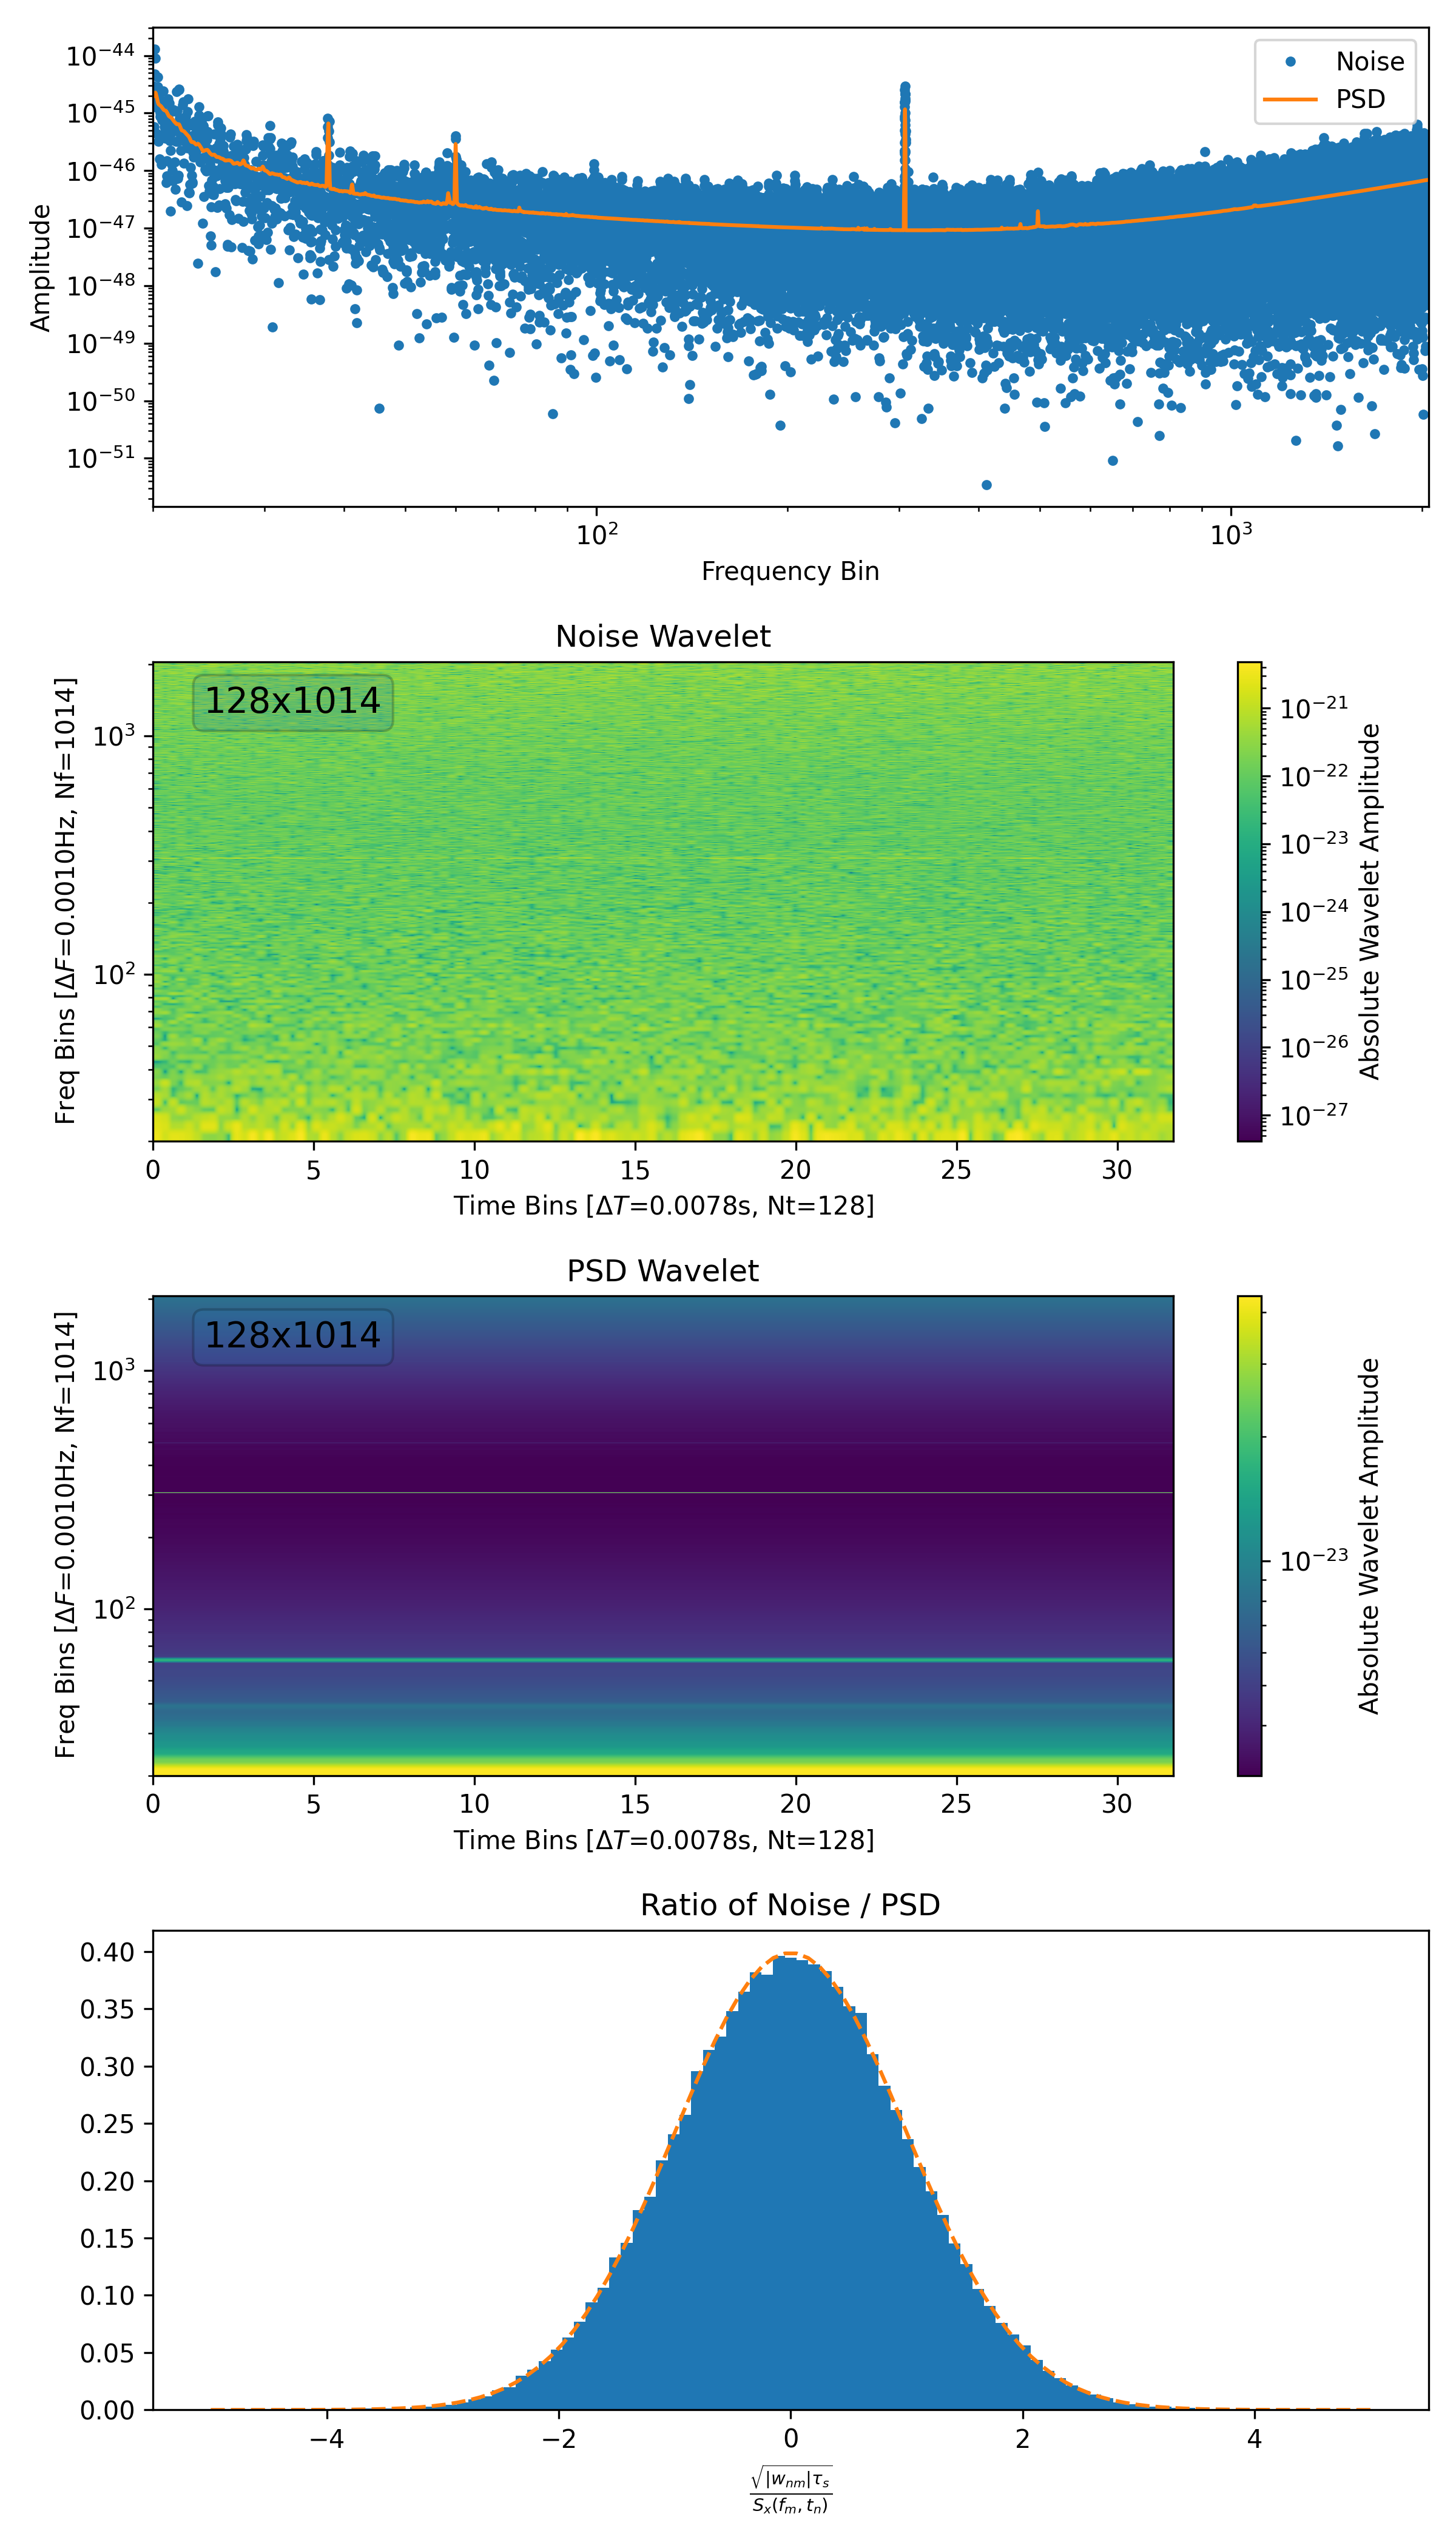
\includegraphics[width=\textwidth]{figures/PSD/lvk_wavelet_psd.png}
    \caption{$S_{\rm LVK}(f)\rightarrow n(\tau_n,f_m)$}
  \end{minipage}
  \hfill
  \begin{minipage}[b]{0.4\textwidth}
    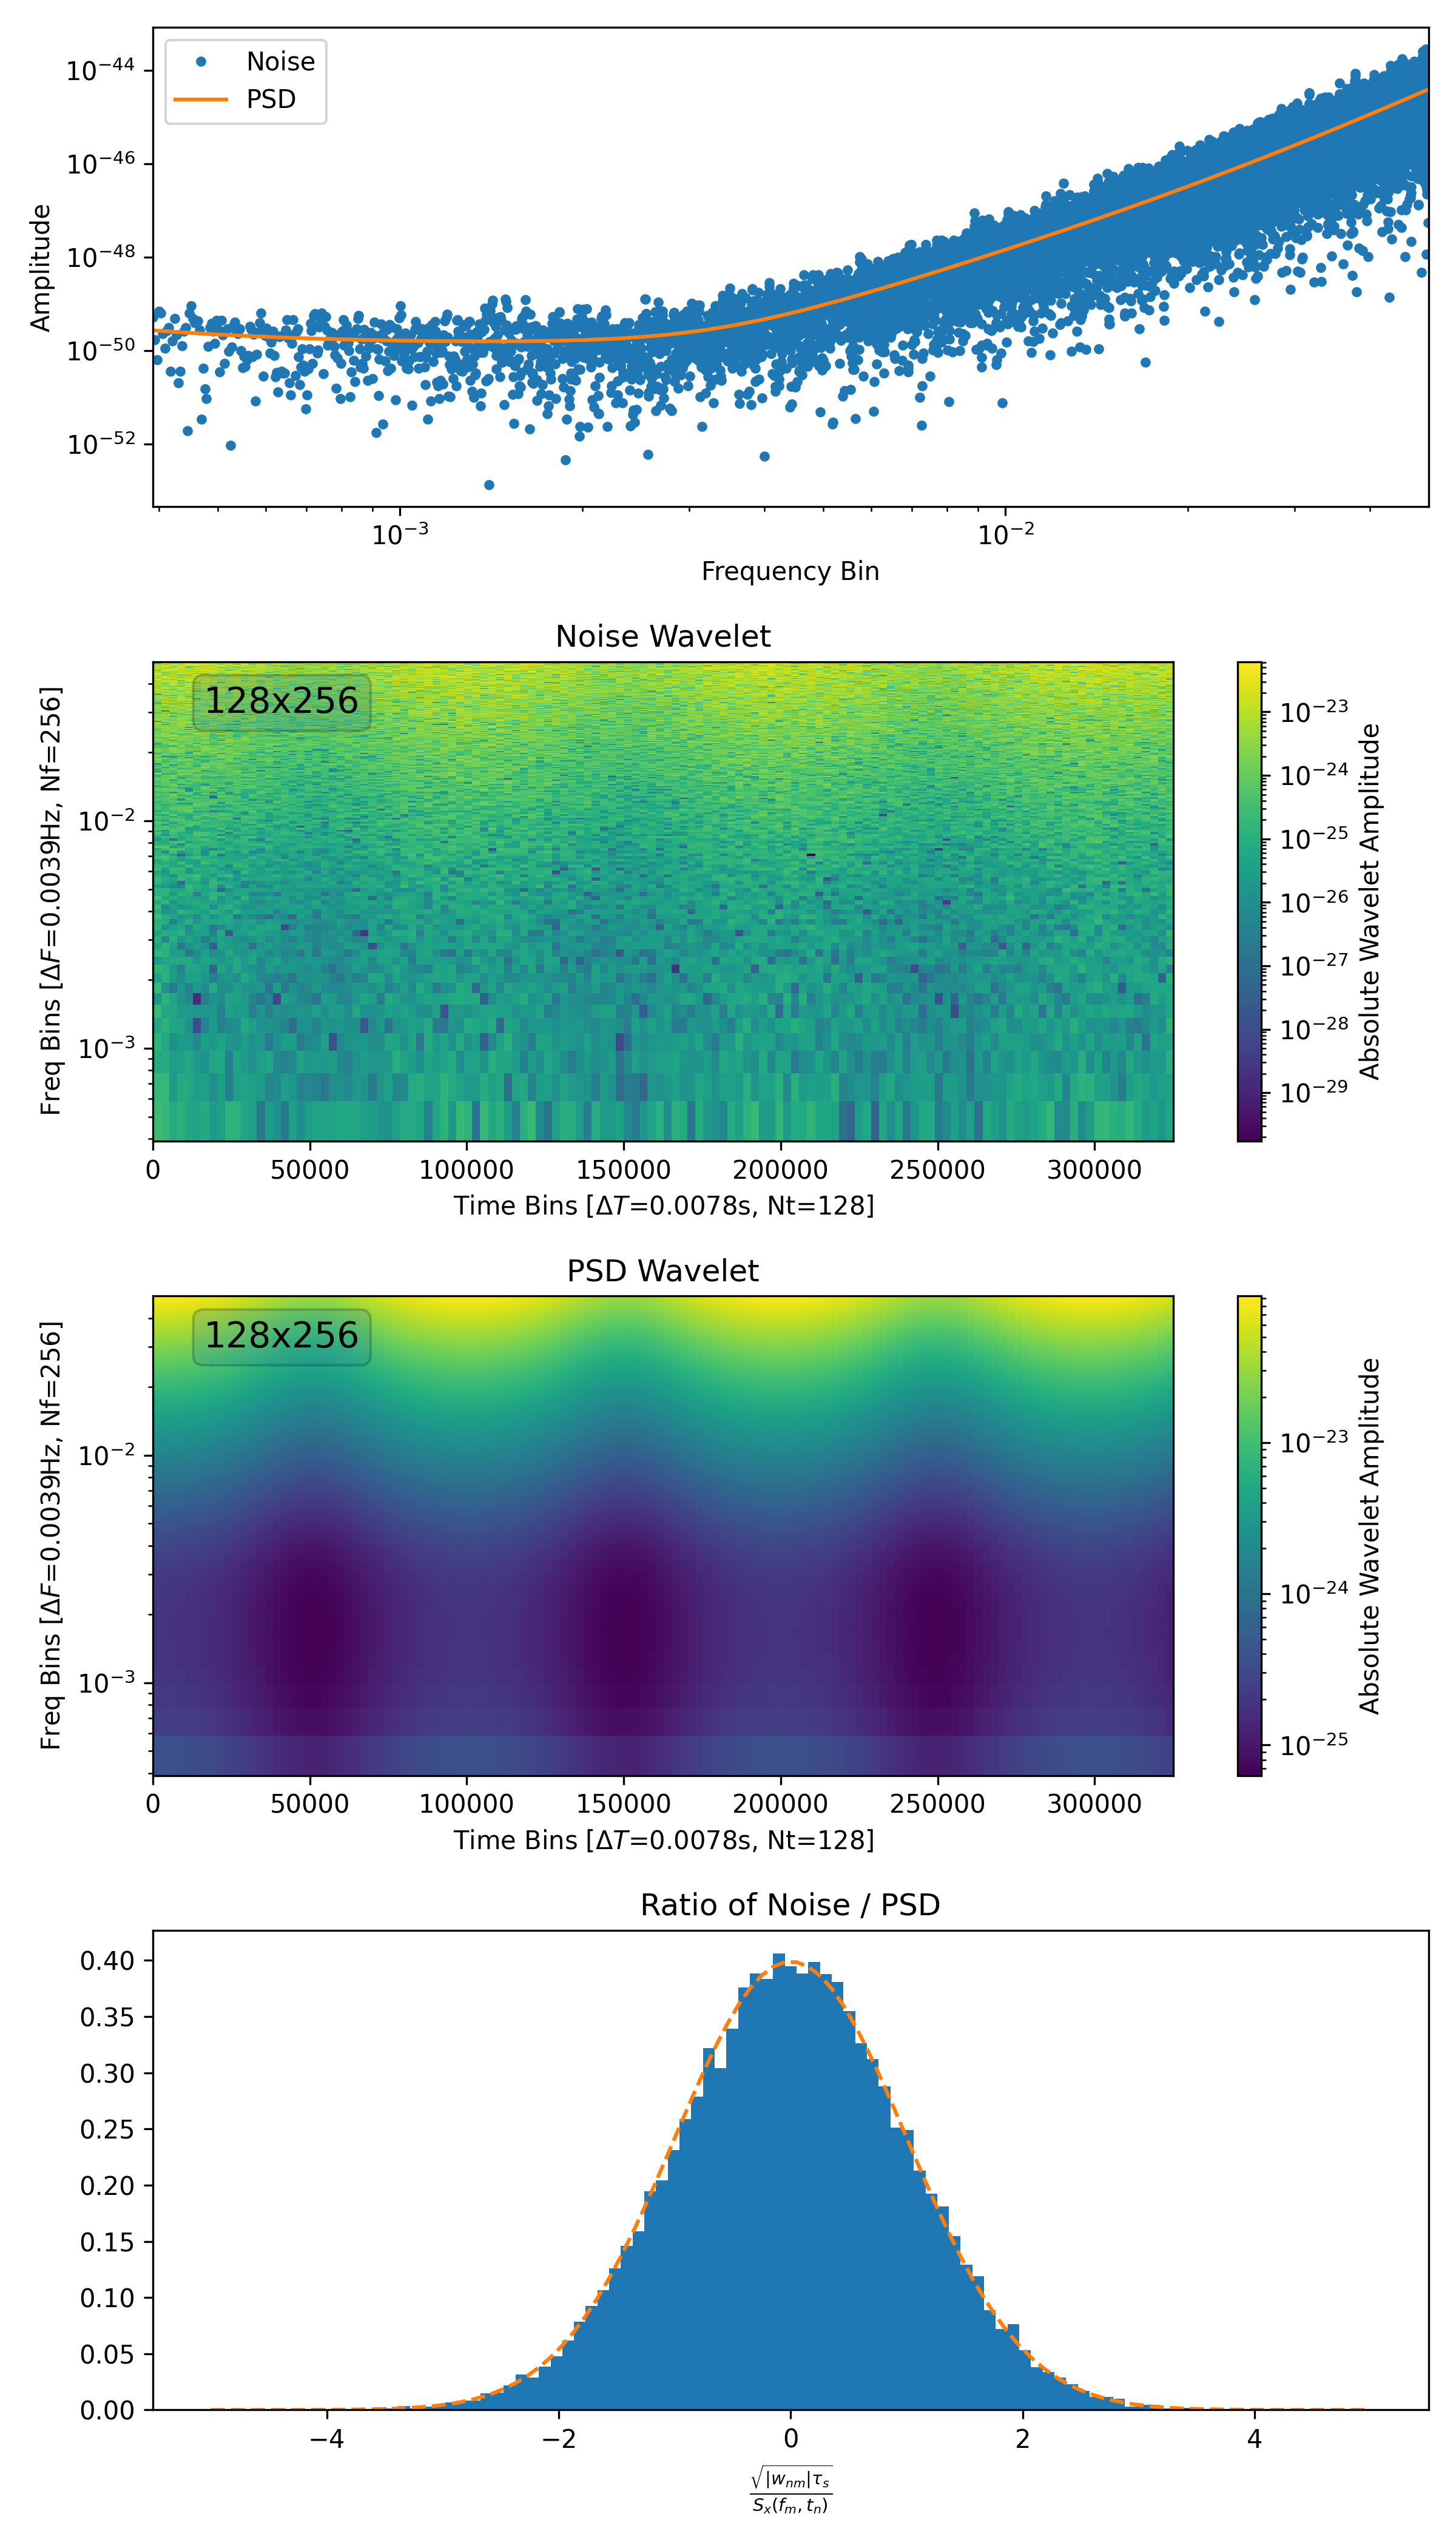
\includegraphics[width=\textwidth]{figures/PSD/lisa_wavelet_modulated_psd.png}
    \caption{$S_{\rm LISA}(f)*a(t)\rightarrow n(\tau_n,f_m)$}
  \end{minipage}
\end{figure}


For the non-stationary PSD, we multiply the stationary PSD $S_n(f)$ and with some time-varying function $g(t)$ leading to an amplitude-modulated spectrum $g(t)S_n(f)$. We can generate a timeseries from the $S_n(f)$, and then multiply the time series with the amplitude modulation ~\cite{nonstationary_psd}

% We now write the $g_{nm}$ as a function of their Fourier transform in the above expression:
% \begin{eqnarray}
%     W_{nm, n'm'} & = & \sum_{k=0}^{N-1} \sum_{k'=0}^{N-1} \int_{-\infty}^{+\infty} \int_{-\infty}^{+\infty} \tilde{g}_{nm}(f) \tilde{g}_{n'm'}(f') e^{2i\pi f k \tau_s} e^{-2i\pi f' k' \tau_s}  R(t_{k}, s_{k'}) \nonumber \\
%     & = & \int_{-\infty}^{+\infty} \int_{-\infty}^{+\infty} \tilde{g}_{nm}(f) \tilde{g}_{n'm'}(f') \sum_{k=0}^{N-1} \sum_{k'=0}^{N-1}   e^{2i\pi (f k - f'k')\tau_s} R(t_{k}, s_{k'}) 
% \end{eqnarray}

\section{Signal-to-noise Ratio}

Cornish states the wavelet SNR is given by
\begin{equation}
    \rho(h) = \sum_{nm} \frac{\hat{h}_{nm}d_{nm}}{S_{nm}}
\end{equation}

The optimal SNR must be:
\begin{equation}
    \rho(h) = \sum_{nm} \frac{h_{nm}h_{nm}}{S_{nm}}
\end{equation}


Refer to A18 from \cite{Veitch:2010:PhRvD} for freq domain SNR


\newpage

\section{GW Data analysis}
\subsection{Wavelet-domain waveforms}
\avi{These are just my notes}

Waveform models such as \textsc{IMRPhenomXPHM}, \textsc{SEOBNRv4PHM} etc are defined in either the time or frequency domain. To analyse data in the wavelet domain, we need waveform models in the wavelet domain. We can do this by:
\begin{enumerate}
    \item Using the equations in Section~\ref{sec:wavelet_domain} to transform time/freq models during analysis. However, this conversion can be costly
    \item Using a surrogate wavelet representation of the waveforms in the wavelet domain.
\end{enumerate}

In the remainder of this section, we discuss two methods of building a surrogate wavelet representation of a waveform.

\subsubsection{Lookup Table wavelet model}
Cornish proposed several methods to obtain waveforms in the wavelet domain, and one was the \textit{lookup-table} method (Section VB, Fast Wavelet Waveforms: Taylor expansion). A GW waveform $h(t, \theta)$ can be written into its phase $\phi(t, \theta)$ and amplitude $A(t,\theta)$ components as 
\begin{align}
h(t,\theta)&=A(t,\theta)\ {\rm exp}[i\Phi(t,\theta)]\,\hspace{2em} {\rm or} \label{eq:ht}\\
h(f,\theta)&=A(f,\theta)\ {\rm exp}[i\tilde{\Phi}(f,\theta)]\,
\end{align}

Taylor expanding the $\Phi(t,\theta)$ about $t=t_n$ gives us:
\begin{alignat}{2}
    \Phi(t,\theta) &= \Phi(t_n, \theta) \nonumber\\
                   &  + \Phi'(t_n, \theta)\ (t - t_n) \nonumber\\
                   &  + \Phi''(t_n, \theta)\ (t - t_n)^2/2! \nonumber\\
                   &  + ... \label{eq:phi_taylor_approx}
\end{alignat}
Similarly, Taylor expanding $A(t, \theta),$
\begin{equation}
    A(t,\theta) = A(t_n) + A'(t_n)(t-t_n) + ...
\end{equation}

Using the \textit{`stationary phase inspired time-frequency mapping'} \avi{Ask where this comes from}:
\begin{alignat*}{2}
\Phi'(t) &= 2\pi f(t) ,\hspace{2em} \tilde{\Phi}'(f) &&= 2\pi t(f) \\
\Phi''(t) &= 2\pi f'(t) ,\hspace{2em} \tilde{\Phi}''(f) &&= 2\pi t'(f) \\
\end{alignat*}
we can rewrite $\phi(t,\theta)$ from Eq~\ref{eq:phi_taylor_approx} as 
\begin{alignat}{2}
    \Phi(t,\theta) &= \Phi(t_n, \theta) \nonumber\\
                   &  + 2\pi f(t_n, \theta)\ (t - t_n) \nonumber\\
                   &  + \pi f'(t_n, \theta)\ (t - t_n)^2 \nonumber\\
                   &  + ... \label{eq:phi_taylor_approx_2} 
\end{alignat}

Rewriting $h(t,\theta)$ Eq.~\ref{eq:ht} using the Taylor expansion (Eq~\ref{eq:phi_taylor_approx_2}) for $\Phi(t,\theta)$,
\begin{align}
    h(t,\theta) &= A(t,\theta)\ {\rm exp}[i\ \Phi(t, \theta)]\\
                &= A(t,\theta)\ {\rm exp}[i ( \Phi(t_n, \theta) + 2\pi f(t_n, \theta)\ (t - t_n) + \pi f'(t_n, \theta)\ (t - t_n)^2)]
\end{align}
     





\subsubsection{Reduced order model:}
Reduced order modeling (ROM) speeds up waveform evaluation in GW astronomy~\cite{2022LRR....25....2T}. To build a reduced order waveform $h_{\rm ROM}(t, \vec{\theta})$, there are two stages:
\begin{enumerate}
    \item Obtaining $\{X_j\}^{Nx}$ `empirical interpolation nodes' (specific time or frequency nodes) for evaluation (the waveform is then generated by interpolating between all $\{X_j\}^{Nx}$).
    \item Generating a basis of waveforms $B=\{h(x,\vec{\theta}_i)\}^{Nb}$ that can be summed up with weights $w_i(t)$ to obtain any other waveform.
\end{enumerate}

The ROM for GW waveform can be given by $h_{\rm ROM}(t,\vec{\theta})=\rm{Interp}[h_{\rm ROM}(x,\vec{\theta})](t)$ can be written as:
\begin{equation}
    h(x,\vec{\theta}) \approx \sum^{\rm \#Basis}_i w_i(\theta) B_i(x)\ ,
\end{equation}
where $B_i(t)$ are the basis, eg $B = \{h(t, \vec{\theta})\}$), and $w_i(t)$ are projection coefficients (weights). The basis can be selected using a greedy approach (iteratively adding the waveform that most improves the overlap between the $h_{\rm ROM}$ and $h_{\rm True}$). Additionally, $w_i(t)$ can be fit using  polynomial interpolation, splines, radial basis, or ML
regression approaches.


In our case, our waveforms will be matrices:

\begin{equation}
    h(x,y,\vec{\theta}) \approx \sum^{\rm \#Basis}_i w_i(\theta) B_i(x,y)\ ,
\end{equation}







\subsection{Likelihood}
Given a time and frequency grid, the Whittle likelihood can be written as 
\begin{equation}
    \mathcal{L}(d|\theta) = -\frac{1}{2}\sum_{t_i,f_j}\left( {\rm ln}(2\pi S[t_i,f_j]) + \frac{d[t_i,f_j] -h(\theta)[t_i,f_j]}{S[t_i,f_j]} \right)
\end{equation}
\avi{However, doesn't this assume that each gridpoint is independent?}


\begin{itemize}
    \item how do different time-freq grids affect the signals' SNR in the wavelet domain?
    \item Generate noise in time and wavelet transform it
    \item Compute the wavelet-SNR + the timeseries SNR
\end{itemize}




\subsection{`Dynamical' whittle likelihood}



\newpage

\section{Analytical derivation of a chirping signal in the wavelet domain}

\subsection{Discrete time-domain Taylor expansion (Giorgio)}

We would like to perform the analytical expression of a chirping signal as the ones used by \url{https://docs.scipy.org/doc/scipy/reference/generated/scipy.signal.chirp.html}, making a comparison with what has been obtained in \url{https://avivajpeyi.github.io/pywavelet/demos/roundtrip_demo.html}. In particular, we set the variable \textit{method='quadratic'}, which means that the signal, in time domain, will be (that's verified numerically)
\begin{align}\label{eq:h_t_cubic}
h(t)=\cos(2\pi\left[f_0t+(f_1-f_0)\frac{t^3}{3t_1^2}\right])
\end{align}
which can be discretized through $t=\frac{T}{N}k$, obtaining the following
\begin{align}\label{eq:h_k}
h[k]=\cos(2\pi\left[f_0\frac{T}{N}k+\frac{(f_1-f_0)}{3t_1^2}\frac{T^3}{N^3}k^3\right])
\end{align}
On the other hand, a good approximation of the Meyer filter is the rectangle function, whose discretized version in the time domain is
\begin{align}
\phi[k]=\textcolor{red}{\frac{1}{\sqrt{2\pi}}}\text{sinc}\left(\frac{\pi k}{2 N_f}\right)
\end{align}
where we remind that both formulas have $k=1\dots N$. Now, given the fact that we suppose the characteristic frequencies in the signal of \eqref{eq:h_k} vary slowly in time, a good approximation of \eqref{eq:h_k} is
\begin{align}
h[nN_f+k]&\simeq\cos(2\pi\varphi_0^n+2\pi\varphi_1^n k)\nonumber\\
\varphi_0^n&=\frac{f_0T}{N_t}n+\frac{f_1-f_0}{3t_1^2}\frac{T^3}{N_t^3}n^3\nonumber\\
\varphi_1^n&=\frac{f_0T}{N}+\frac{f_1-f_0}{t_1^2}\frac{T^3}{N_t^3N_f}n^2
\end{align}
And then using
\eqref{eq:direct} we obtain
\begin{align}
w_{n m}&=\sqrt{2} \frac{T}{N} \Re \left[C_{n m} \sum_{k=-qN_f}^{qN_f-1} e^{i \pi k m / N_f} h\left[n N_f+k\right] \phi[k]\right]=\nonumber\\
&=\sqrt{2} \frac{T}{N} \Re \left[C_{n m} \sum_{k=-qN_f}^{qN_f-1} e^{i \pi k m / N_f}\cos\left(2\pi\varphi_0^n+2\pi\varphi_1^n k\right)\frac{1}{\sqrt{2\pi}}\text{sinc}\left(\frac{\pi k}{2 N_f}\right)\right]=\nonumber\\
&=\frac{T}{N} \Re \left[C_{n m} \sum_{k=-qN_f}^{qN_f-1} e^{i \pi k m / N_f}\frac{e^{2\pi i\varphi_0^n+2\pi i\varphi_1^n k}+c.c.}{2}\frac{1}{\sqrt{\pi}}\frac{e^{i\frac{\pi k}{2 N_f}}-c.c.}{i\frac{\pi k}{N_f}}\right]=\nonumber\\
&=\frac{T}{N_t2\pi\sqrt{\pi}} \Im \left[C_{n m} \sum_{k=-qN_f}^{qN_f-1} e^{i \pi k m / N_f}\left(e^{2\pi i\varphi_0^n+2\pi i\varphi_1^n k}+c.c.\right)\frac{e^{i\frac{\pi k}{2 N_f}}-c.c.}{k}\right]=\nonumber\\
&= \frac{T}{N_t2\pi\sqrt{\pi}} \Im \Bigg[C_{n m} e^{2\pi i\varphi_0^n}\sum_{k=-qN_f}^{qN_f-1}\frac{1}{k}\left(e^{2\pi i\left(\varphi_1^n+\frac{1}{4N_f}+\frac{m}{2N_f}\right) k}-e^{2\pi i\left(\varphi_1^n-\frac{1}{4N_f}+\frac{m}{2N_f}\right) k}\right)+\nonumber\\
&+C_{n m} e^{-2\pi i\varphi_0^n}\sum_{k=-qN_f}^{qN_f-1}\frac{1}{k}\left(e^{2\pi i\left(-\varphi_1^n+\frac{1}{4N_f}+\frac{m}{2N_f}\right) k}-e^{2\pi i\left(-\varphi_1^n-\frac{1}{4N_f}+\frac{m}{2N_f}\right) k}\right)\Bigg]=\nonumber\\
&=\frac{T}{N_t2\pi\sqrt{\pi}} \Im \Bigg[C_{n m} \cos(2\pi\varphi_0^n)\frac{2\pi i}{N_f}
\end{align}
\textcolor{red}{Last equation is work in progress...}

\subsection{Continuous time-domain Taylor expansion (Quentin)}

\subsubsection{General case}

Like Giogio above, we start from Eq.~\eqref{eq:direct}
\begin{equation}
w_{n m}=\sqrt{2} \Delta t \Re \left[C_{n m} \sum_{k=-K / 2}^{K / 2-1} e^{2\pi i k m q / K} x\left[n N_f+k\right] \phi[k]\right].
\end{equation}
where $K = 2q N_f$ is the width of the window function and $q$ determines the size of the window relative to the time resolution of the time-frequency pixels.
% Note that from Eqs.\eqref{wnm_def} and \eqref{eq:gnm} this is equivalent to 
% \begin{eqnarray}
% w_{n m} &=& \sum_{k=0}^{N-1} x[k] g_{nm}[k] \nonumber \\
% & = & \sum_{k=0}^{N-1} x[k] e^{- i n \omega_k \Delta T}\left(C_{nm}\tilde\phi(\omega_k -m\Delta\Omega)+C^{*}_{nm}\tilde\phi(\omega_k +m\Delta\Omega)\right).
% \end{eqnarray}
% where $\omega_k = 2 \pi \frac{k f_s}{N}$

Note that using the continuous approximation, the wavelet transform is essentially a convolution with the shifted window function:
\begin{eqnarray}
\label{eq:wavelet_transform_continuous}
    w_{n m} \approx \sqrt{2} \Delta t \Re \left\{C_{n m} \int_{-\infty}^{+\infty} e^{2 \pi i t f_{mq}} x(n \Delta T + t) \phi(t) dt\right\},
\end{eqnarray}
where we use the following definitions the fact that $\Delta T = N_f \tau_s$ and we set $f_{mq} = \frac{mq}{K}f_s$. 

\begin{eqnarray}
  \Delta T = N_f \tau_s \label{eq:dT_tau}\\
  f_{mq} = \frac{mq}{K}f_s\label{eq:fmq}
\end{eqnarray}




Owing to the window function symmetry, we have equivalently:
\begin{eqnarray}
\label{eq:wavelet_transform_continuous_sym}
    w_{n m} \approx \sqrt{2} \Delta t \Re \left\{C_{n m} \int_{-\infty}^{+\infty} e^{-2 \pi i t f_{mq}} x(n \Delta T - t) \phi(t) dt\right\},
\end{eqnarray}
Let us write the signal as
\begin{eqnarray}
\label{eq:time_waveform_amp_phase}
    x(t) = \Re\left\{A(t) e^{i \Psi(t)} \right\} = \frac{1}{2}A(t)\left(e^{i \Psi(t)} + e^{-i \Psi(t)}\right)
\end{eqnarray}
Let's assume that $A(t)$ evolves slowly with time, and let's Taylor-expand the phase:
\begin{eqnarray}
\label{eq:time_waveform_expansion}
    \Psi(n\Delta T + t) \approx \Psi(n\Delta T) + t \dot{\Psi}(n\Delta T) + \frac{1}{2} t^2 \ddot{\Psi}(n\Delta T)
\end{eqnarray}
Plugging Eqs.~\eqref{eq:time_waveform_amp_phase} and \eqref{eq:time_waveform_expansion} into Eq.~\eqref{eq:wavelet_transform_continuous} we get
\begin{eqnarray}
\label{eq:wavelet_transform_continuous_expansion}
    w_{n m} & \approx & \sqrt{2} \Delta t \Re C_{n m} A(t_n) e^{i\Psi(n\Delta T)} \int_{-\infty}^{+\infty} e^{-2 \pi i t f_{mq}} e^{i\left(t \dot{\Psi}(n\Delta T) + \frac{1}{2} t^2 \ddot{\Psi}(n\Delta T)\right)}\phi(t) dt, \nonumber \\
    && + \sqrt{2} \Delta t \Re C_{n m} A(t_n) e^{-i\Psi(n\Delta T)} \int_{-\infty}^{+\infty} e^{-2 \pi i t f_{mq}} e^{-i\left(t \dot{\Psi}(n\Delta T) + \frac{1}{2} t^2 \ddot{\Psi}(n\Delta T)\right)}\phi(t) dt.
\end{eqnarray}
Let's consider the first part for now, since the second line can be derived from the first one by complex conjugation and some minus signs.
\begin{eqnarray}
    w_{n m} & \approx & \sqrt{2} \Delta t \Re C_{n m} \frac{1}{2}A(t_n) e^{i\Psi(n\Delta T)} \int_{-\infty}^{+\infty} e^{-2 \pi i t\left( f_{mq} - \nu(n\Delta T)\right)} e^{i \pi  t^2 \dot{\nu}(n\Delta T)}\phi(t) dt \nonumber \\
    && + \sqrt{2} \Delta t \Re C_{n m} \frac{1}{2} A(t_n) e^{-i\Psi(n\Delta T)} \int_{-\infty}^{+\infty} e^{-2 \pi i t\left( f_{mq} + \nu(n\Delta T)\right)} e^{-i \pi  t^2 \dot{\nu}(n\Delta T)}\phi(t) dt
\end{eqnarray}
where we set 
\begin{eqnarray}
    \nu(t) \equiv \frac{1}{2 \pi} \dot{\Psi}(t).
\end{eqnarray}
Note that if we ignore the second-order term, we get:
\begin{eqnarray}
\label{eq:wavelet_time_approx_first_order}
    w_{n m} & \approx & \sqrt{2} \Delta t \Re C_{n m} \frac{1}{2} A(t_n) \left[ e^{i\Psi(n\Delta T)} \tilde{\phi}\left( f_{mq} - \nu(n\Delta T) \right) + e^{-i\Psi(n\Delta T)} \tilde{\phi}^{\ast}\left( f_{mq} + \nu(n\Delta T) \right)\right]
\end{eqnarray}

\subsubsection{Example of a chirp}
Let us consider the signal:
\begin{equation}
    x(t) = \cos\left( 2 \pi f_0 t + a t^{2} \right).
\end{equation}
for which we have 
\begin{eqnarray}
    \Psi(t) & = & 2 \pi f_0 t + a t^{2} \nonumber \\
    \nu(t) & = & 2 \pi f_0 + 2 a t \nonumber \\
    \dot{\nu}(t) & = & 2a
\end{eqnarray}
\textcolor{red}{Isn't the second line $\nu(t) = f_0 + \frac{2 a t}{2 \pi}$ and the third $\dot\nu(t) =\frac{2 a}{2 \pi}$ ?}
We can restrict the wavelet coefficient equation Eq if we consider only positive frequencies $f_{mq}$.~\eqref{eq:wavelet_time_approx_first_order} to
\begin{eqnarray}
\label{eq:wavelet_time_approx_first_order_tsquared}
    w_{n m} & \approx & \sqrt{2} \Delta t \Re C_{n m} \frac{1}{2} A(t_n) e^{i\Psi(n\Delta T)} \tilde{\phi}\left( f_{mq} - f_0 - \frac{a t_n}{\pi} \right)
\end{eqnarray}
% The window function is non-zero for frequencies such that $|f_{mq} - \nu(t_n)| \leq \frac{\Delta F}{2}$ and zero otherwise. This is equivalent to
% \begin{eqnarray}
%      \left| \frac{mq}{K} - \frac{f_0}{f_s} - \frac{2 a n \Delta T}{\pi f_s} \right|  \leq \frac{\Delta F}{2f_s}
% \end{eqnarray}

\subsubsection{The $t^3$ chirp (Giorgio)}
We start from \eqref{eq:wavelet_time_approx_first_order} and \eqref{eq:h_t_cubic} where now
%
\begin{align}
    \Psi(t) &= 2 \pi f_0 t + a t^{3}\nonumber\\
    \nu(t) &= f_0 + \frac{3 a}{2\pi} t^2\nonumber\\
    a&=2\pi \frac{f_1-f_0}{3t_1^2}
\end{align}
%
obtaining
%
\begin{align}
\label{eq:wavelet_time_approx_first_order_tcube}
w_{n m} \approx \sqrt{2} \Delta t \Re C_{n m} \frac{1}{2} A(t_n) e^{i\Psi(n\Delta T)} \tilde{\phi}\left( f_{mq} - f_0 - \frac{3a t_n^2}{2\pi} \right)
\end{align}

\subsection{Frequency-domain Taylor expansion}

Let us consider an arbitrary function of time $x(t)$ whose Fourier transform is $X(f)$.

The expression of the wavelet transform of $x$ involves the expression of $x_m$ in Eq.~\ref{eq:wdft}, whose continuous version can be expressed as
\begin{align}
\label{eq:wdft-continuous}
    x(f_m, \tau_n) = \int_{-\infty}^{+\infty} e^{-2\pi i f \tau_n} X(f+ f_m)\tilde{\phi}(f) df,
\end{align}
where we set $f_m = m N_t/2 f_s$ and $\tau_n = n \tau_s$.
The frequency window $\tilde{\phi}(f)$ represented in Fig.~\ref{fig:phi_omega} restricts the frequencies contributing to the integral to the bandwidth $\Delta F$ around the central frequency $s$. 
The frequency-domain waveform can be split in amplitude and phase:
\begin{eqnarray}
\label{eq:amplitude_phase_split}
    X(f) = A(f) e^{i\Theta(f)}
\end{eqnarray}
Therefore, we can Taylor both amplitude and phase:
\begin{eqnarray}
    A(f + f_m) &=& A(f_m) + f A'(f_m) + ... \\
    \Theta(f + f_m) &=& \Theta(f_m) + f \Theta'(f_m) + \frac{1}{2} f^2 \Theta''(f_m)
\end{eqnarray}
Plugging this approximation into Eq.~\eqref{eq:wdft-continuous} yields
\begin{align}
\label{eq:wdft-continuous-taylor}
    x(f_m, \tau_n) & = \int_{-\infty}^{+\infty} e^{-2\pi i f \tau_n} \tilde{\phi}(f) A(f_m) e^{i \left(\Theta(f_m) + f \Theta'(f_m) + \frac{1}{2} f^2 \Theta''(f_m)\right)} df \nonumber \\
    & + \int_{-\infty}^{+\infty} e^{-2\pi i f \tau_n} \tilde{\phi}(f) \textcolor{red}{f} A'(f_m) e^{i\left(\Theta(f_m) + f \Theta'(f_m) + \frac{1}{2} f^2 \Theta''(f_m)\right)} df
\end{align}
For now, we will keep only the leading order in amplitude and concentrate on the phase expansion. We can take some terms out of the integral.
\begin{align}
\label{eq:wdft-continuous-taylor-2}
    x(f_m, \tau_n) & = A(f_m) e^{i\Theta(f_m)} \int_{-\infty}^{+\infty} \tilde{\phi}(f)  e^{-2\pi i f \tau_n} e^{i \left(f \Theta'(f_m) + \frac{1}{2} f^2 \Theta''(f_m)\right)} df 
\end{align}
which is amazing as it shows we can construct wavelet templates from frequency-domain waveforms and their derivatives. Of course, we can extend this decomposition to arbitrary precision. 

\subsubsection{Numerical approach}

From Eq.~\eqref{eq:wdft-continuous-taylor-2} we see that computing the wavelet coefficients requires valuating quantities depending on the frequency phase derivatives:
\begin{eqnarray}
\label{eq:definition_enm}
e_{nm} \equiv \int_{-\infty}^{+\infty} \tilde{\phi}(f)  e^{-2\pi i f \tau_n} e^{i \left(f \Theta'(f_m) + \frac{1}{2} f^2 \Theta''(f_m)\right)} df.
\end{eqnarray}
Let's approximate them with a discrete Fourier transform:
\begin{eqnarray}
e_{nm} \approx \frac{f_s}{N_t}\sum_{k=0}^{N_t-1} \tilde{\phi}(f_k)  e^{-2\pi i k n / N_t} e^{i \left(f_k \Theta'(f_m) + \frac{1}{2} f_k^2 \Theta''(f_m)\right)}.
\end{eqnarray}
where $f_k = k f_s / N_t$ are the Fourier frequencies corresponding to the wavelet time grid.
This way, we can use the fast Fourier transform algorithm to comptue the DFT of 
\begin{eqnarray}
    \tilde{e}_{nm}(k) \equiv \tilde{\phi}(f_k) e^{i \left(f_k \Theta'(f_m) + \frac{1}{2} f_k^2 \Theta''(f_m)\right)}.
\end{eqnarray}


\subsubsection{Analytical approach}

Cornish argues that one can use the stationary phase approximation, where there is a map between time and frequency as:
\begin{eqnarray}
    f & \longrightarrow & t(f) = \frac{1}{2 \pi} \frac{d\Theta(f)}{df} \\
    t & \longrightarrow & f(t) = \frac{1}{2 \pi} \frac{d\Psi(t)}{dt} 
\end{eqnarray}


Let us define the function
\begin{eqnarray}
    \tilde{z}(f) \equiv \tilde{\phi}(f) e^{i\frac{1}{2} f^2 \Theta''(f_m)}
\end{eqnarray}
Then the equation \eqref{eq:wdft-continuous-taylor-2} can be written as a function of the inverse Fourier transform of $\tilde{z}(f)$, that we label as $z(t)$:
\begin{align}
\label{eq:wdft-continuous-taylor-3}
    x(f_m, \tau_n) & = A(f_m) e^{i\Theta(f_m)} z\left(\tau_n - \frac{\Theta'(f_m)}{2 \pi} \right),
\end{align}
where
\begin{eqnarray}
\label{eq:z_inverse_fourier}
    z(t) = \int_{-\infty}^{+\infty}\tilde{z}(f) e^{-2\pi i f t} df.
\end{eqnarray}

\subsubsection{First-order}
It is interesting to note that up to first order in the phase, we get

\begin{align}
\label{eq:wdft-continuous-taylor-first-order}
    x(f_m, \tau_n) \approx X(f_m) \phi\left(\tau_n - \frac{\Theta'(f_m)}{2 \pi} \right).
\end{align}

\subsubsection{Second-order}

To simplify the computation, we consider that the window function $\tilde{\phi}(f)$ is approximately rectangular so that
\begin{align}
\label{eq:meyer_window_freq_approx}
\tilde\phi(\omega) \approx \left\{\begin{array}{lr}
\frac{1}{\sqrt{2 \pi \Delta F }} & |f| < \frac{\Delta F}{2}\\
0 & \text{otherwise.}
\end{array}\right.\;,
\end{align}
Then the integral in Eq.~\eqref{eq:z_inverse_fourier} can be approximated as
\begin{align}
\label{eq:z_inverse_fourier-2}
    z(t) & = \frac{1}{\sqrt{2 \pi \Delta F }} \int_{-\Delta F/2}^{+\Delta F/2} e^{i\frac{1}{2} f^2 \Theta''(f_m)} e^{-2\pi i f t} df
\end{align}
 With Mathematica, we derive that 
\begin{eqnarray}
    z(t) & = & \frac{1}{\sqrt{2 \pi \Delta F }} \left[I_{\frac{\Delta F}{2}}(t) - I_{-\frac{\Delta F}{2}}(t)  \right] 
\end{eqnarray}
with
\begin{eqnarray}
    I_{T}(t) & = & -\frac{1}{2} \sqrt{\frac{\pi}{a}} e^{i\frac{3 \pi}{4} - i \frac{\pi^2 t^2}{a}} \operatorname{erfi}\left( e^{i\frac{\pi}{4}} \frac{aT - \pi t}{\sqrt{a}}\right)
\end{eqnarray}
where $\operatorname{erfi}$ is the imaginary error function and $a = \frac{1}{2} \Theta''(f_m)$.

Then, we simply need to apply Eq.~\eqref{eq:fast}:
\begin{align}
\label{eq:fast-2}
    w_{nm} & =\sqrt{2}(-1)^{nm}\Re\left[C_{nm} x(f_m, \tau_n)\right] \nonumber \\
\end{align}

\subsubsection{Example of a chirp}
Let us assume that the analysed signal is a chirp of the form 

\begin{equation}
\label{eq:chirp-time}
    x(t) = \cos\left( 2 \pi f_0 t + a t^{2} \right).
\end{equation}
We can decompose it as 
\begin{equation}
\label{eq:chirp-time-decomposed}
    x(t) = \cos\left( 2 \pi f_0 t \right) \cos\left(a t^{2} \right) - \sin\left( 2 \pi f_0 t \right) \sin\left(a t^{2} \right).
\end{equation}
The Fourier transform of the quadratic terms are 
\begin{eqnarray}
   \tilde{c}_{2}(f) \equiv \mathcal{F}\left[\cos\left(a t^{2} \right)\right](f) & =&  \sqrt{\frac{\pi}{a}} \cos\left(\frac{\pi^2 f^2}{a} - \frac{\pi}{4} \right) \nonumber \\
   \tilde{s}_{2}(f) \equiv \mathcal{F}\left[\sin\left(a t^{2} \right)\right](f) & =&  - \sqrt{\frac{\pi}{a}} \sin\left(\frac{\pi^2 f^2}{a} - \frac{\pi}{4} \right) 
\end{eqnarray}
So we can write the Fourier transform of \eqref{eq:chirp-time-decomposed} as
\begin{eqnarray}
    X(f) & = & \frac{1}{2}\left(\tilde{c}_{2}(f-f_0) + \tilde{c}_{2}(f+f_0)\right) \nonumber \\
    & &  - \frac{1}{2i}\left(\tilde{s}_{2}(f-f_0) - \tilde{s}_{2}(f+f_0)\right) \nonumber \\
    & = & \frac{1}{2}\left(\tilde{e}(f-f_0) + \tilde{e}(f+f_0)^{\ast}\right)
\end{eqnarray}
where we defined
\begin{eqnarray}
    \tilde{e}(f) & \equiv & \tilde{c}(f) + i \tilde{s}(f) \nonumber \\
    & = & \sqrt{\frac{\pi}{a}} e^{-i \left(\frac{\pi^2 f^2}{a} - \frac{\pi}{4} \right)}
\end{eqnarray}
Let us concentrate on the positive frequency part. By identification with Eq.~\eqref{eq:amplitude_phase_split}, we have
\begin{eqnarray}
    A(f) & = & \frac{1}{2}\sqrt{\frac{\pi}{a}} \nonumber \\
    \Theta(f) & = & \frac{\pi}{4} - \frac{\pi^2 (f-f_0)^2}{a} \nonumber \\
    \Theta'(f) & = & - \frac{2 \pi^2 (f-f_0)}{a} \nonumber \\
    \Theta''(f) & = & - \frac{2 \pi^2}{a}
\end{eqnarray}

% In our example, we have
% \begin{equation}
%     \tilde{e}(f) = \frac{1}{2}\sqrt{\frac{\pi}{a}} \exp\left\{ i \left(\frac{\pi^2 f^2}{a} - \frac{\pi}{4} \right) \right\}.
% \end{equation}
% From the definition of $C_{nm}$ we have
% \begin{align}
% \label{eq:fast-3}
%     w_{nm} & = \sqrt{2}(-1)^{nm}\Re\left[x_m(n)\right] \, \text{ if } n + m \text{ is even} \nonumber \\
%      & = - \sqrt{2}(-1)^{nm}\Im\left[x_m(n)\right] \, \text{ if } n + m \text{ is odd}
% \end{align}


\section{GW detector response in the wavelet domain}

Here we examine the possibility of performing template-free GW searches in LISA data.

\subsection{As a function of the wavelet-domain GW waveform}
The detector's response to an incoming gravitational wave depends on its location in the sky, or equivalently, on its wave vector $\hat{\mathbf{k}}$. In LISA, it also depends on time (as the constellation moves around the Sun during the observation) and on the source's frequency. The link response to a particular polarization $p$ is therefore written as a convolution 
\begin{eqnarray}
y_{l m, p}(t, \hat{\mathbf{k}}) \approx & \frac{1}{2\left(1-\hat{\mathbf{k}} \cdot \hat{\mathbf{n}}_{l m}(t)\right)}\left[ 
 h_p\left(t-\frac{L_{l m}(t)}{c}-\frac{\hat{\mathbf{k}} \cdot \mathbf{x}_m(t)}{c}, \hat{\mathbf{n}}_k\right) 
-h_p\left(t-\frac{\hat{\mathbf{k}} \cdot \mathbf{x}_l(t)}{c}, \hat{\mathbf{n}}_k\right)\right] \xi_p\left(\hat{\mathbf{u}}_k, \hat{\mathbf{v}}_k, \hat{\mathbf{n}}_{l m}\right) .
\end{eqnarray}
where $h_p$ in the wave strain amplitude for polarization $p$ and $\xi_p$ are the modulation functions of the antenna pattern.
Let's set 
\begin{eqnarray}
    F_{lm, p}(t, \hat{\mathbf{k}}) & \equiv & \frac{1}{2\left(1-\hat{\mathbf{k}} \cdot \hat{\mathbf{n}}_{l m}(t)\right)} \xi_p\left(\hat{\mathbf{u}}_k, \hat{\mathbf{v}}_k, \hat{\mathbf{n}}_{l m}\right) \\ 
    \tau^{r}_{lm}(t, \hat{\mathbf{k}}) & \equiv & \frac{L_{l m}(t)}{c}-\frac{\hat{\mathbf{k}} \cdot \mathbf{x}_m(t)}{c}\\
    \tau^{e}_{lm}(t, \hat{\mathbf{k}}) & \equiv & \frac{\hat{\mathbf{k}} \cdot \mathbf{x}_l(t)}{c}.
\end{eqnarray}
For now, let us drop the link indices $l, m$ and polarization $p$ indices for clarity.
For each link and polarization, we thus have
\begin{eqnarray}
\label{eq:response_simple}
y(t, \hat{\mathbf{k}}) \approx & F(t, \hat{\mathbf{k}}) \cdot \left[ 
 h\left(t-\tau^{r}(t), \hat{\mathbf{k}}\right) -h\left(t-\tau^{e}(t), \hat{\mathbf{k}} \right) \right].
\end{eqnarray}
Now, we can decompose the time-domain GW perturbation in the wavelet basis, from Eq.~\eqref{eq:inverse_wavelet_decomposition}
\begin{align}
\label{eq:inverse_wavelet_decomposition_2}
h(t_k) = \sum_{n=0}^{N_t-1}\sum_{m=0}^{N_f-1}h_{nm}g_{nm}(t_k).
\end{align}
Let's first plug this expression into Eq.~\eqref{eq:response_simple}
\begin{eqnarray}
\label{eq:response_simple_decomp}
y(t, \hat{\mathbf{k}}) \approx & F(t, \hat{\mathbf{k}}) \sum_{n'=0}^{N_t-1}\sum_{m'=0}^{N_f-1}h_{n'm'}(\hat{\mathbf{k}}) \left[ 
 g_{n'm'}\left(t-\tau^{r}(t)\right) -g_{n'm'}\left(t-\tau^{e}(t))\right) \right].
\end{eqnarray}
Transforming the response into the wavelet domain gives
\begin{align}
\label{response_wavelet}
W[y]_{nm} & = \sum_{k=0}^{N-1} g_{nm}(t_k) y(t_k, \hat{\mathbf{k}}) \nonumber \\
& =  \sum_{n'=0}^{N_t-1}\sum_{m'=0}^{N_f-1}h_{n'm'}(\hat{\mathbf{k}}) \sum_{k=0}^{N-1}  g_{nm}(t_k)  F(t_k, \hat{\mathbf{k}})  \left[ 
 g_{n'm'}\left(t_k-\tau^{r}(t_k)\right) -g_{n'm'}\left(t_k-\tau^{e}(t_k))\right) \right]
\end{align}
Let us define the kernel
\begin{eqnarray}
\label{eq:kernel_def}
    k_{n'm'}(t) \equiv F(t, \hat{\mathbf{k}})  \left[ 
 g_{n'm'}\left(t-\tau^{r}(t)\right) -g_{n'm'}\left(t-\tau^{e}(t)\right) \right],
\end{eqnarray}
and its wavelet transform $W[k_{n'm'}]_{nm}$. We get:
\begin{align}
\label{response_wavelet_2}
W[y]_{nm} = \sum_{n'=0}^{N_t-1}\sum_{m'=0}^{N_f-1}h_{n'm'}(\hat{\mathbf{k}}) W[k_{n'm'}]_{nm}
\end{align}
Hence, we can write the response as a function of the GW signal's and kernel's wavelet transforms. The question is now: can we approximate the kernel in the wavelet domain, as we do in the frequency domain?

Some remarks:
\begin{itemize}
    \item The modulation functions $F(t, \hat{\mathbf{k}})$ evolves slowly with the orbital motion, and so do the delays $\tau^{r}$ and $\tau^{e}$.
    \item The basis functions involved in the kernel are well defined in the frequency domain \item The components $g_{nm}(t)$ are localized in time-frequency around frequency $f_m$ and time $t_n$.
    \item It's tempting to use the orthonormality condition $\sum_{k=0}^{N-1}g_{nm}(t_k)g_{n'm'}(t_k) = \delta_{nn'}\delta_{mm'}$.
\end{itemize}

The wavelet transform of the kernel reads
\begin{eqnarray}
\label{eq:kernel_wavelet_transform}
    W[k_{n'm'}]_{nm} = \sum_{k=0}^{N-1} g_{nm}(t_k) k_{n'm'}(t_k).
\end{eqnarray}
We assume that the modulation function $F(t, \hat{\mathbf{k}})$ an the delays $\tau(t)$ evolve slowly in time with respect to the wavelet resolution.
Then for $|t - t_n| \leq \Delta T$ we can write
\begin{eqnarray}
\label{eq:kernel_approx}
    k_{n'm'}(t) \approx F(t_n, \hat{\mathbf{k}})  \left[ 
 g_{n'm'}\left(t-\tau^{r}(t_n)\right) -g_{n'm'}\left(t-\tau^{e}(t_n)\right) \right],\, \forall t \text{ s.t. } |t - t_n| \leq \Delta T
\end{eqnarray}
The function $g_{n'm'}(t)$ is localized around $t_{n'}$, so for a constant delay we have
\begin{eqnarray}
g_{n'm'}(t - \tau^{r}(t_n)) \approx g_{n'-q^{r}[n],m'}(t),
\end{eqnarray}
where $q^{r}[n] = \lfloor \tau^{r}(t_n) / \Delta T \rfloor$.
Plugging Eq.~\eqref{eq:kernel_approx} into Eq.~\eqref{eq:kernel_wavelet_transform}, we get
\begin{eqnarray}
\label{eq:kernel_wavelet_transform_approx}
    W[k_{n'm'}]_{nm} & \approx & F(t_n, \hat{\mathbf{k}}) \sum_{k=0}^{N-1} g_{nm}(t_k) 
    \left[ g_{n'-q^{r}[n], m'}(t_k) - g_{n'-q^{e}[n], m'}(t_k) \right] \nonumber \\
    & = & F(t_n, \hat{\mathbf{k}}) \delta_{mm'} \left[ \delta_{n, n'-q^{r}[n]} - \delta_{n, n'-q^{e}[n]}\right]
\end{eqnarray}
Let's now go back to the response in the wavelet domain in Eq.~\eqref{response_wavelet}. We inject the approximation of Eq.~\eqref{eq:kernel_wavelet_transform_approx} to find
\begin{align}
\label{response_wavelet_approx}
W[y]_{nm} & \approx  \sum_{n'=0}^{N_t-1}\sum_{m'=0}^{N_f-1}h_{n'm'}(\hat{\mathbf{k}}) W[k_{n'm'}]_{nm} \nonumber \\
& =  F(t_n, \hat{\mathbf{k}})  \sum_{n'=0}^{N_t-1}\sum_{m'=0}^{N_f-1}h_{n'm'} \delta_{mm'} \left[ \delta_{n, n'-q^{r}[n]} - \delta_{n, n'-q^{e}[n]}\right] \nonumber \\
& = F(t_n, \hat{\mathbf{k}}) \left[ h_{n+q^{r}[n], m} - h_{n+q^{e}[n], m}\right].
\end{align}
Which is what we wanted: an expression of the GW response in the wavelet domain as a function of the wavelet transform of the GW strain signal. 

\subsection{As a function of the frequency-domain GW waveform}

To get a form similar as in the frequency domain response, we can express the wavelet transform as a function of the window function.
For any signal $x$ we have
\begin{eqnarray}
    W[x]_{nm} &=& \sum_{k=0}^{N-1} g_{nm}(t_k) x(t_k) \nonumber \\
              &=& \sum_{k=0}^{N-1} \int_{-\infty}^{+\infty} \tilde{\phi}_{m}(f) e^{2 \pi i f (t_k-n \Delta T)} x(t_k) df \nonumber \\
              & = & \int_{-\infty}^{+\infty} \tilde{\phi}_{m}(f) e^{-2 \pi i f n \Delta T} \sum_{k=0}^{N-1} x(t_k) e^{2 \pi i f t_k} df \nonumber \\
              & = & \int_{-\infty}^{+\infty} \tilde{\phi}_{m}(f)  \tilde{x}(f)^{\ast} e^{-2 \pi i f n \Delta T}df
\end{eqnarray}
where we defined $\phi_{m}$ as the inverse Fourier transform of $\tilde{\phi}_{m}(f) \equiv C_{nm}\tilde\phi(f-m\Delta F)+C^*_{nm}\tilde\phi(f+m\Delta F )$.

Using this form in the wavelet-domain response in Eq.~\eqref{response_wavelet_approx} yields
\begin{align}
\label{response_wavelet_approx_freq}
W[y]_{nm} & \approx F(t_n, \hat{\mathbf{k}}) \int_{-\infty}^{+\infty} \tilde{\phi}_{m}(f) \tilde{h}(f)^{\ast}  \left[ e^{-2 \pi i f q^{r}[n] \Delta T} - e^{-2 \pi i f q^{e}[n] \Delta T}\right] e^{-2 \pi i f n \Delta T} df \nonumber \\
& = \int_{-\infty}^{+\infty} \tilde{h}(f)^{\ast} \tilde{G}(n, m, f) df.
\end{align}
Defining the frequency-domain kernel
\begin{eqnarray}
    \tilde{G}(n, m, f) \equiv  F(t_n, \hat{\mathbf{k}}) \tilde{\phi}_{m}(f)  \left[ e^{-2 \pi i f q^{r}[n] \Delta T} - e^{-2 \pi i f q^{e}[n] \Delta T}\right] e^{-2 \pi i f n \Delta T}
\end{eqnarray}

% \begin{align}
% \tilde{g}_{mn}(f) = e^{-2\pi i n\Delta T f}\left(C_{nm}\tilde\phi(f-m\Delta F)+C^*_{nm}\tilde\phi(f+m\Delta F )\right)
% \end{align}
% We have 
% \begin{eqnarray}
%     g_{nm}(t) &=& \int_{-\infty}^{+\infty} \tilde{g}_{mn}(f) e^{2 \pi i f t} df \nonumber \\
%     & = & \int_{-\infty}^{+\infty} \left(C_{nm}\tilde\phi(f-m\Delta F)+C^*_{nm}\tilde\phi(f+m\Delta F )\right) e^{2 \pi i f (t-n \Delta T)} df \nonumber \\
%     & = & \int_{-\infty}^{+\infty} \tilde{\phi}_{m}(f) e^{2 \pi i f (t-n \Delta T)} df \nonumber \\
%     & = & \phi_{m}(t-n \Delta T)
% \end{eqnarray}
% where we defined $\phi_{m}$ as the inverse Fourier transform of $\tilde{\phi}_{m}(f) \equiv C_{nm}\tilde\phi(f-m\Delta F)+C^*_{nm}\tilde\phi(f+m\Delta F )$.
% The kernel in Eq.~\eqref{eq:kernel_def} can then be expressed as
% \begin{eqnarray}
% \label{eq:kernel_vs_frequency}
%     k_{n'm'}(t) & = &  F(t, \hat{\mathbf{k}}) \int_{-\infty}^{+\infty} \tilde{\phi}_{m}(f) e^{2 \pi i f (t-n' \Delta T)} \left[ e^{-2 \pi i f \tau^{r}(t)} - e^{-2 \pi i f \tau^{e}(t)} \right] \nonumber \\
%     & = & F(t, \hat{\mathbf{k}}) \left[\phi_{m}(t-n \Delta T - \tau^{r}(t)) - \phi_{m}(t-n \Delta T - \tau^{e}(t)) \right]
% \end{eqnarray}

% By plugging the above expression into Eq.~\eqref{eq:inverse_wavelet_decomposition_2} we have
% \begin{eqnarray}
%     h(t) &=& \sum_{n=0}^{N_t-1}\sum_{m=0}^{N_f-1} h_{nm} \phi_{m}(t-n \Delta T) \nonumber \\
%     & = & \sum_{n=0}^{N_t-1}\sum_{m=0}^{N_f-1} h_{nm} \int_{-\infty}^{+\infty} \tilde{\phi}_{m}(f) e^{2 \pi i f (t-n \Delta T)}
% \end{eqnarray}
% We can plug this decomposition into the response \eqref{eq:response_simple}
% \begin{eqnarray}
% \label{eq:response_simple_2}
% y(t, \hat{\mathbf{k}}) &\approx & F(t, \hat{\mathbf{k}}) \sum_{n=0}^{N_t-1}\sum_{m=0}^{N_f-1} h_{nm}(\hat{\mathbf{k}})  \int_{-\infty}^{+\infty}  \tilde{\phi}_{m}(f) e^{2 \pi i f (t-n \Delta T)}
% \left[ e^{- 2 \pi i f \tau^{r}(t)} - e^{-2 \pi i f \tau^{e}(t)} \right] df. \nonumber \\
% \end{eqnarray}
% We define the following convolution kernel:
% \begin{eqnarray}
%    G_{nm}(f, t, \hat{\mathbf{k}}) \equiv F(t, \hat{\mathbf{k}}) \tilde{\phi}_{m}(f) e^{-2 \pi i f n \Delta T}  \left[ e^{- 2 \pi i f \tau^{r}(t)} - e^{-2 \pi i f \tau^{e}(t)} \right]
% \end{eqnarray}
% to simplify the equation as
% \begin{eqnarray}
% \label{eq:response_simple_3}
% y(t, \hat{\mathbf{k}}) &\approx & \sum_{n=0}^{N_t-1}\sum_{m=0}^{N_f-1} h_{nm}(\hat{\mathbf{k}})  \int_{-\infty}^{+\infty} e^{2 \pi i f t} G_{nm}(f, t, \hat{\mathbf{k}}) df. \nonumber \\
% \end{eqnarray}




% \begin{eqnarray}
% \label{eq:link_response_time}
%     y_{l m, p}(t, \hat{\mathbf{k}}) \approx \int_{-\infty}^{+\infty} \tilde{h}_p(f^{\prime}, \hat{\mathbf{k}}) e^{2 \pi i f^{\prime} t} G_{l m, p}(f^{\prime}, t, \hat{\mathbf{k}}) \mathrm{d} f^{\prime},
% \end{eqnarray}
% , and $G_{l m, p}$ is a convolution kernel defining the antenna pattern.
% For now, let us drop the link indices $l, m$ and polarization $p$ indices for clarity.
% For each link and polarization, we thus have
% \begin{eqnarray}
% \label{eq:link_response_time_simple}
%     y(t, \hat{\mathbf{k}}) \approx \int_{-\infty}^{+\infty} \tilde{h}(f^{\prime}, \hat{\mathbf{k}}) e^{2 \pi i f^{\prime} t} G(f^{\prime}, t, \hat{\mathbf{k}}) \mathrm{d} f^{\prime}.
% \end{eqnarray}
%We would like to write Eq.~\eqref{eq:link_response_time} in the wavelet domain. 
%By linearity, we have
% \begin{eqnarray}
% \label{eq:link_response_wavelet_simple}
%     w_{mn} &=& \sum_{k=0}^{N-1} y(t_k, \hat{\mathbf{k}}) g_{nm}[k]\nonumber \\
%     & = & \int_{-\infty}^{+\infty} \tilde{h}(f^{\prime}, \hat{\mathbf{k}}) e^{2 \pi i f^{\prime} t} \sum_{k=0}^{N-1}  g_{nm}[k] G(f^{\prime}, t_k, \hat{\mathbf{k}}) \mathrm{d} f^{\prime}.
% \end{eqnarray}

\appendix

\section{Notes}

\avi{Putting some notes here for reference}

\begin{figure}
  \centering

  \begin{subfigure}{0.5\textwidth}
    \centering
    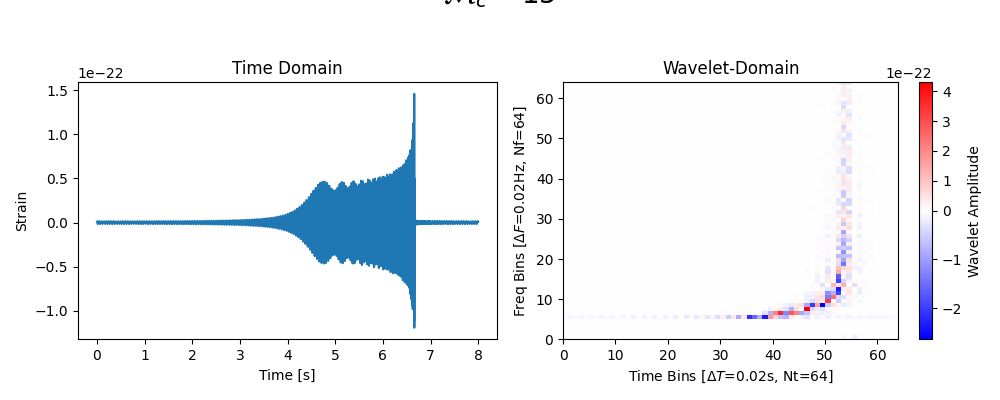
\includegraphics[width=\linewidth]{figures/cbc_imrphenom_d/cbc_wavelet_mc_15.png}
    \caption{$\mathcal{M}_c=15\ M_{\odot}$}
  \end{subfigure}

  \begin{subfigure}{0.5\textwidth}
    \centering
    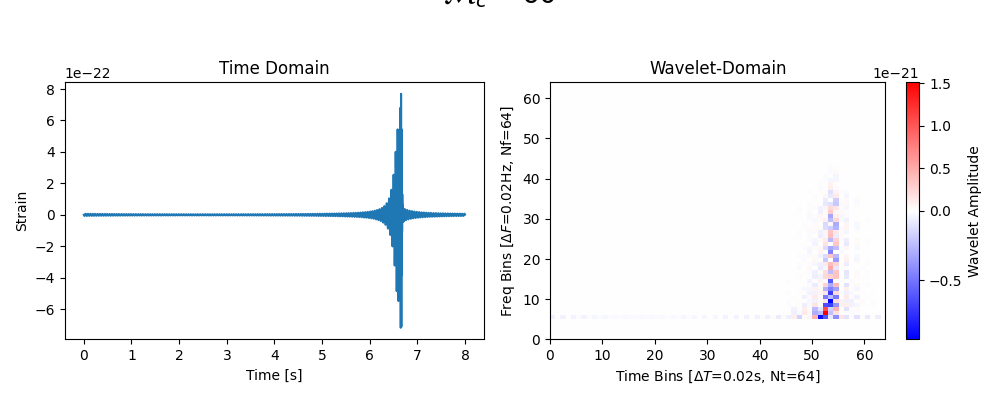
\includegraphics[width=\linewidth]{figures/cbc_imrphenom_d/cbc_wavelet_mc_60.png}
    \caption{$\mathcal{M}_c=60\ M_{\odot}$}
  \end{subfigure}

  \caption{Two CBC GW signals in time and wavelet domain. \avi{This plots' wavelet time and freq are bins: what time and frequencies do the bins correspond to?} \href{https://github.com/avivajpeyi/pywavelet/blob/main/docs/demos/cbc_demo.ipynb}{Link to code}.}
\end{figure}


\begin{figure}
  \centering

  \begin{subfigure}{0.5\textwidth}
    \centering
    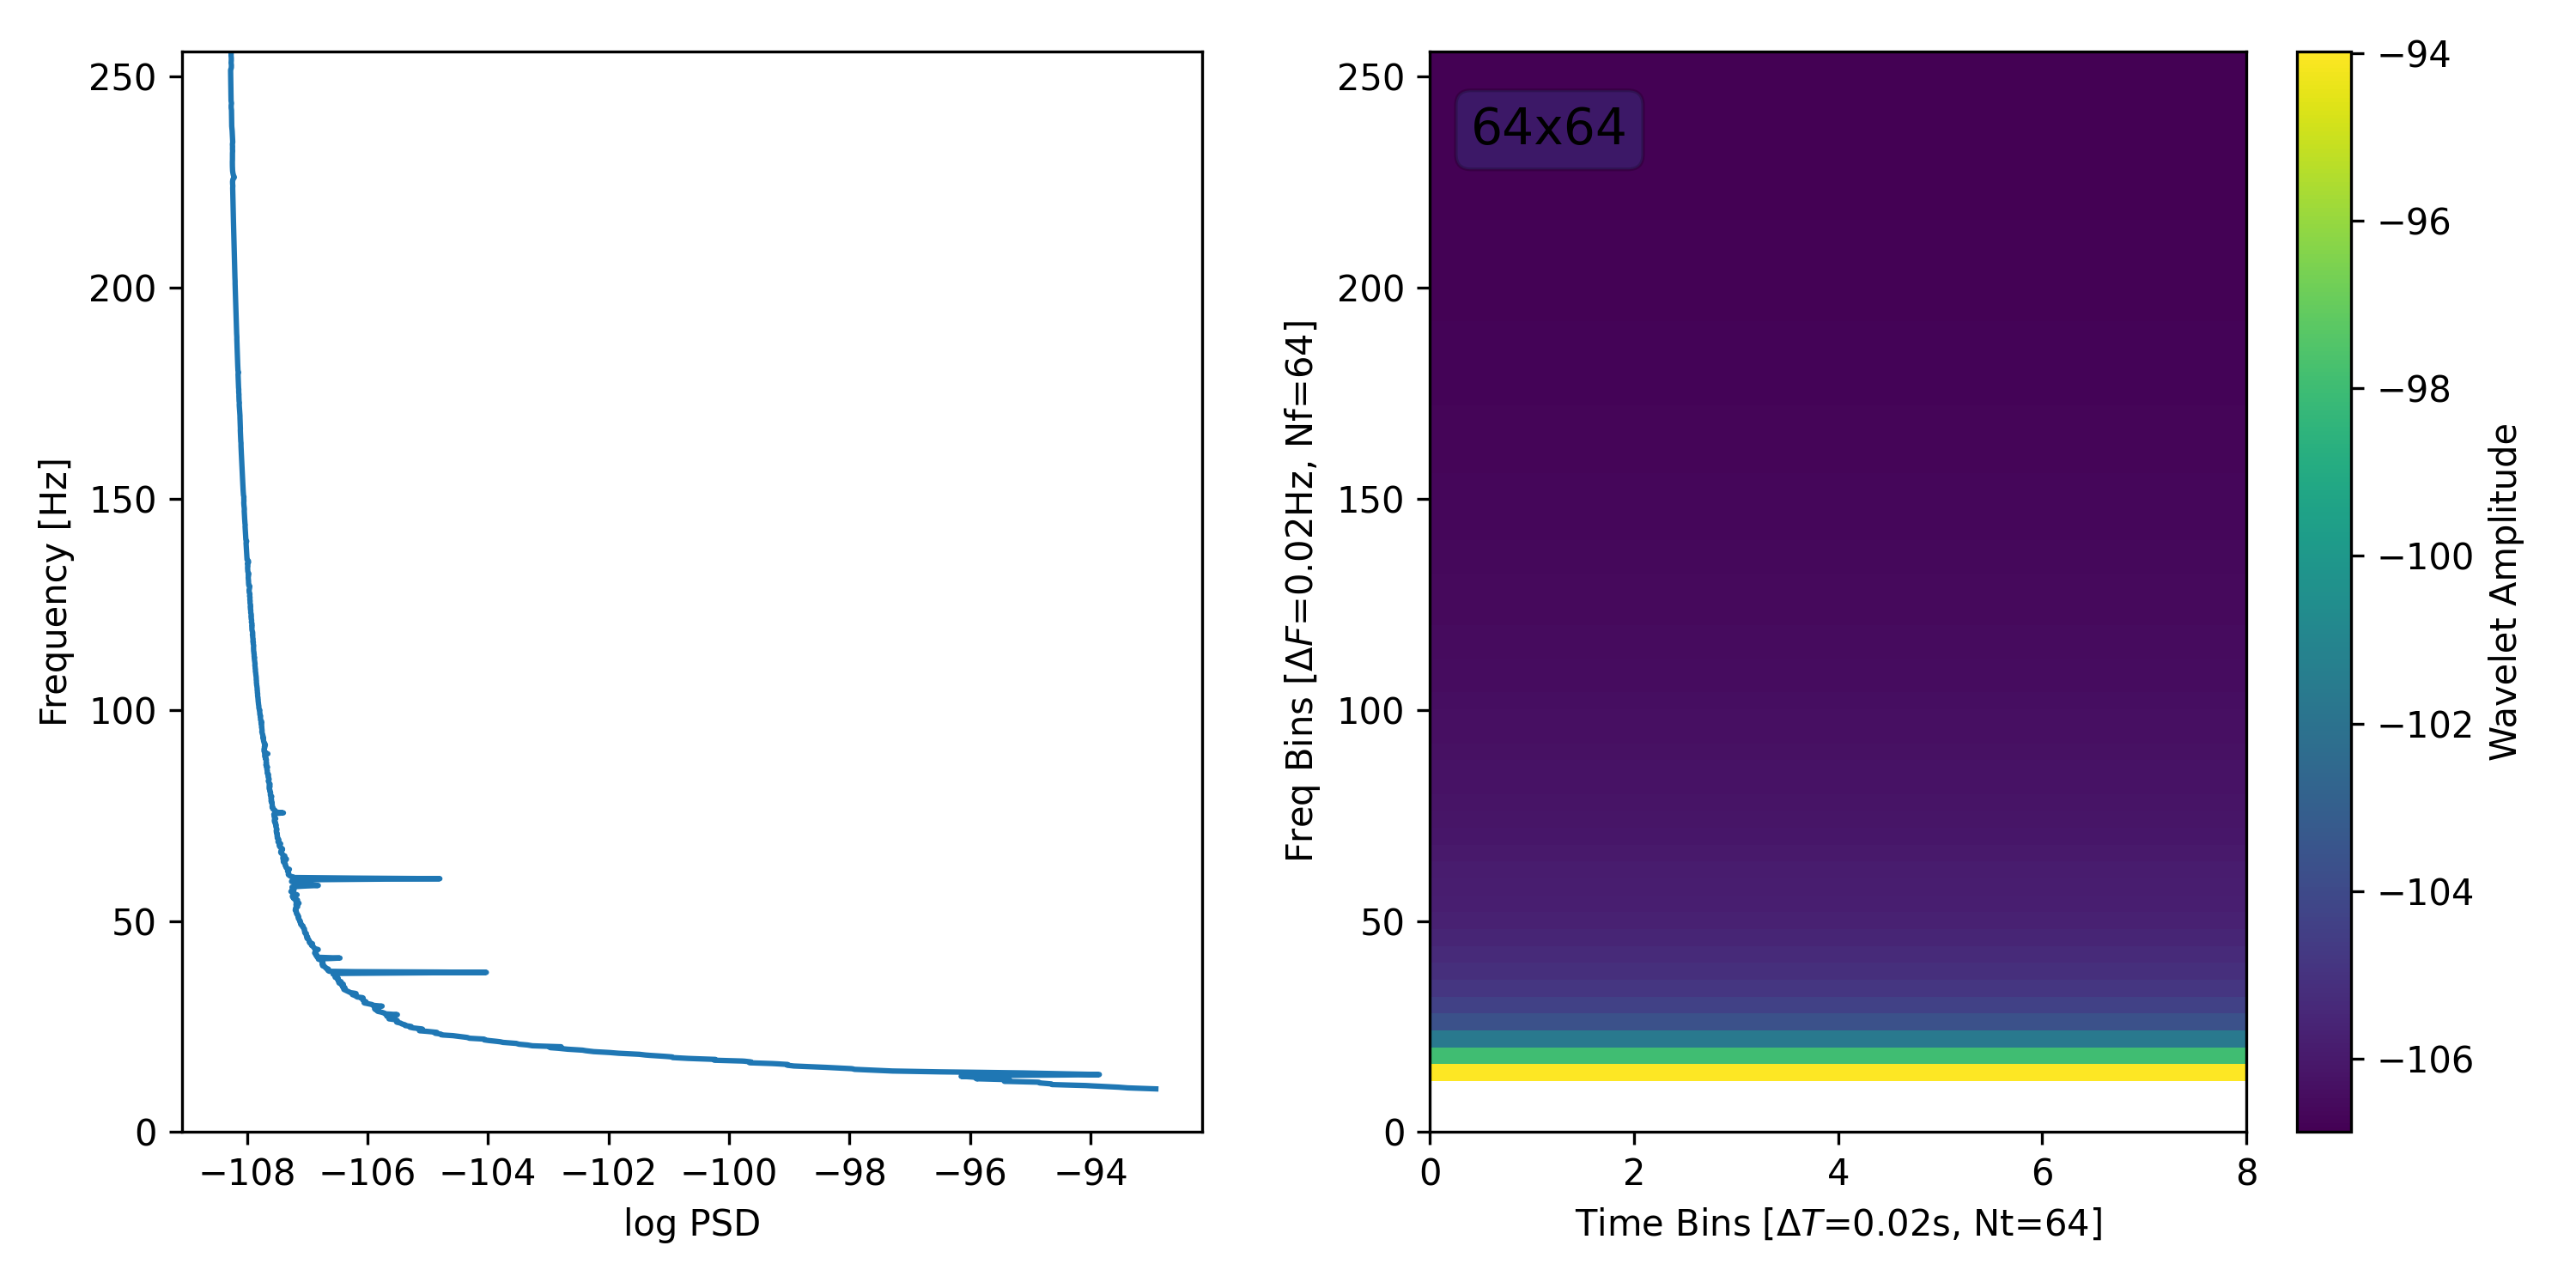
\includegraphics[width=\linewidth]{figures/PSD/psd_wavelet_64.png}
    \caption{$N_f=64$}
  \end{subfigure}

  \begin{subfigure}{0.5\textwidth}
    \centering
    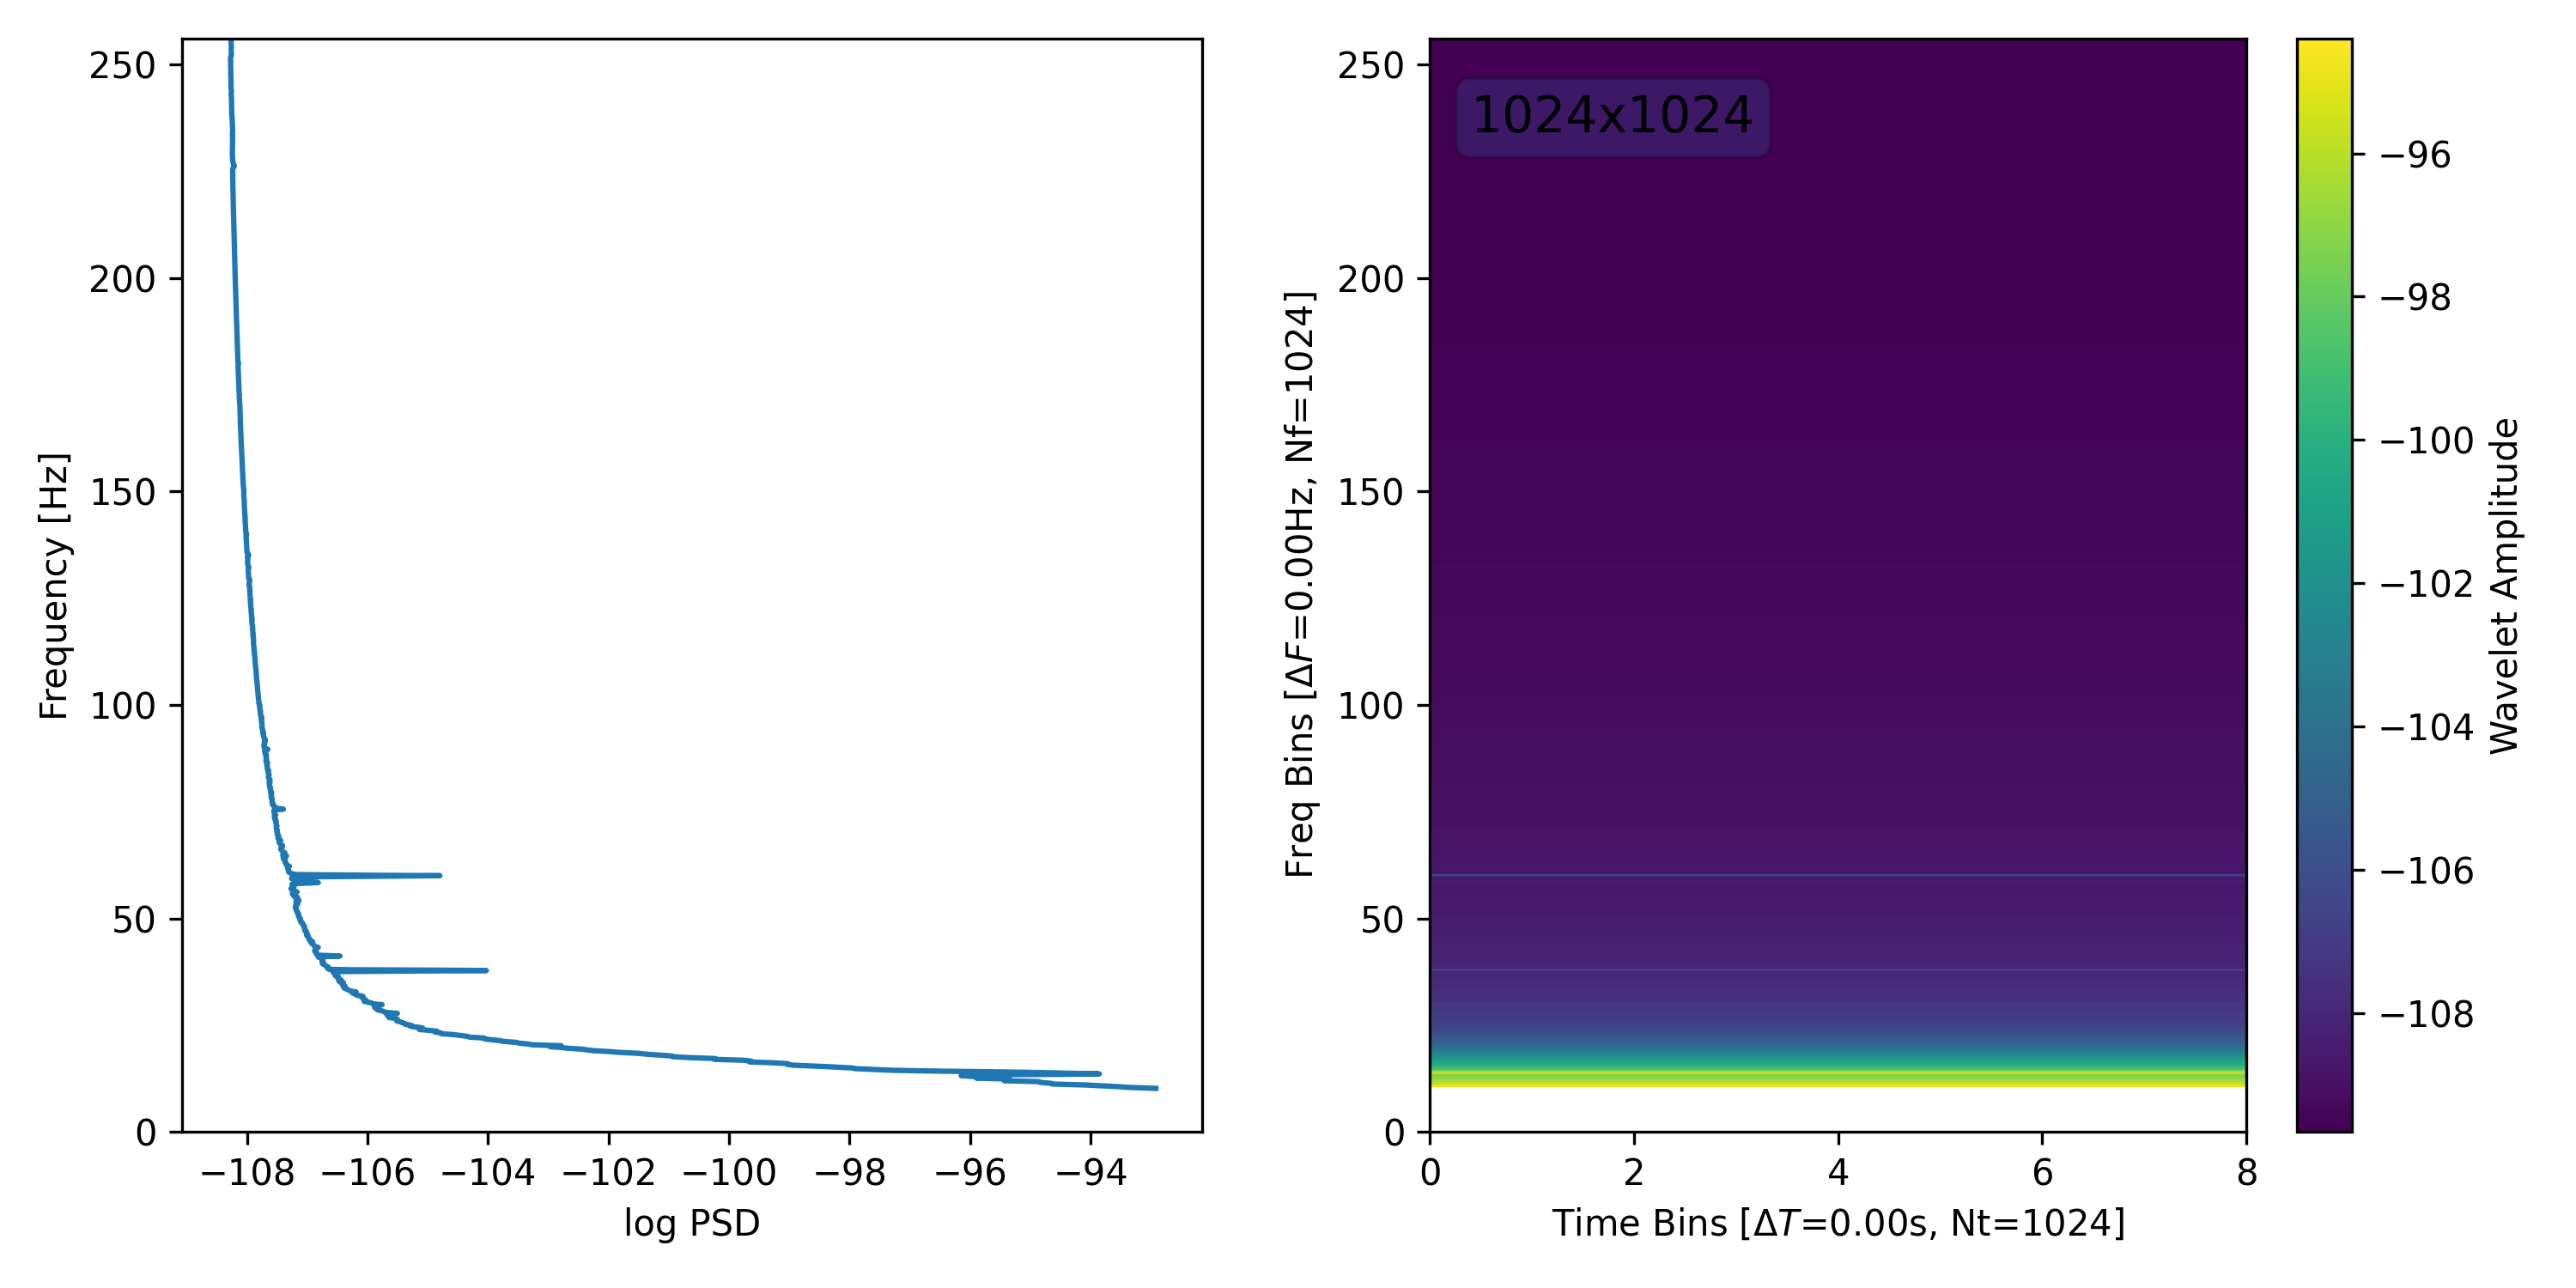
\includegraphics[width=\linewidth]{figures/PSD/psd_wavelet_1024.png}
    \caption{$N_f=1024$}
  \end{subfigure}

  \caption{Example of an evolutionary PSD generated from a stationary PSD using and different bin sizes. Note that some violin modes ($f\sim32, 64$ Hz) are not visible when using $N_f=64$ bins. \href{https://github.com/avivajpeyi/pywavelet/blob/main/tests/test_psd.py}{Link to code}.}
\end{figure}

\newpage
\section{PSD in wavelet domain [Giorgio]}
It took me a while to get familiar with the definitions of PSD, strain, etc, so I write it there for reference. A good reference in my opinion is \url{https://arxiv.org/abs/1408.0740}.
Let's consider ground-based instruments for simplicity since the generalization to the space-based ones is almost straightforward. In the \textbf{time} domain, each interferometer has a data stream
\begin{align}
s(t)&=h(t)+n(t)\nonumber\\
h(t)&=h_{ab}(t,\vec x)d^{ab}
\end{align}
where $h_{ab}(t,\vec x)$ is the time-dependent GW tensor, and $d^{ab}$ is the arm tensor.
The PSD lives in the time domain, therefore we introduce the Fourier-transformed data stream
\begin{align}
\tilde s(f)=\int_0^Tdt' s(t)\,e^{2\pi i f t'}\equiv \tilde h(f)+\tilde n(f)
\end{align}
with T the \textbf{total} observation time. And the PSD of the noise $S(f)$ is defined through the equation
\begin{align}\label{PSD_def_cont}
\langle \tilde n(f)\tilde n^*(f')\rangle=\frac 1 2 \delta(f-f')S(f)
\end{align}
where angle brackets $\langle\cdot\rangle$ denote an ensemble average over many noise realisations\footnote{We can assume ergodicity, therefore this can be translated into the average of the many measurements during the duration of the experiment}. A couple of observations are necessary:
\begin{itemize}
    \item $s(t)$ is adimensional, $\tilde s(f)$ has the dimension of a time
    \item $S(f)$ has the dimension of a time
    \item $S(f)$ is exactely the one plotted in \url{http://gwplotter.com/} as "Power Spectral Density". Please note it is plotted as a sqrt
\end{itemize}

\subsection{Simplified statistics of the wavelets}
We start from Eq.~\eqref{eq:direct}
\begin{equation}
w_{n m}=\sqrt{2} \Delta t \Re \left[C_{n m} \sum_{k=-K / 2}^{K / 2-1} e^{2\pi i k m q / K} x\left[n N_f+k\right] \phi[k]\right].
\end{equation}
where $K = 2q N_f$ is the width of the window function and $q$ determines the size of the window relative to the time resolution of the time-frequency pixels. We recall that we can approximate
\eqref{eq:wavelet_transform_continuous}
%
\begin{align}
w_{n m} &\approx \sqrt{2} \Re \left\{C_{n m} \int_{-\infty}^{+\infty} e^{2 \pi i t f_{m}} x(n \Delta T + t) \phi(t) dt\right\}=\nonumber\\
&=\sqrt{2} \Re \left\{C_{n m} \int_{-\infty}^{+\infty}dt\int_{-\infty}^{+\infty}df' e^{2 \pi i t (f_{m}-f)} e^{-2 \pi i n\Delta T f} \tilde x(f) \phi(t)\right\}
\end{align}
%
with $f_{m} = m\frac{f_{max}}{N_f}=m\frac{N}{2\,T\,N_f}=\frac{m}{2\Delta T}$. Here we used $dt=\Delta t$ to go to the continuous limit. Let's forget of the $\Re$ operator so far and let's compute the wavelet statistics for the noise $\tilde n(f)$, making use of \eqref{PSD_def_cont},
%
\begin{align}
\langle w_{n m}w_{n'm'}\rangle&\simeq C_{n m}C_{n'm'}\int dt\phi(t) \int dt' \phi(t')\int df e^{2 \pi i t (f_{m}-f)} e^{-2 \pi i (n-n')\Delta T f} e^{2 \pi i t' (f_{m'}-f)} S(f)\simeq\nonumber\\
&\simeq C_{n m}C_{nm'}\int dt\phi(t) \int dt' \phi(t')\int df e^{2 \pi i t (f_{m}-f)} e^{2 \pi i t' (f_{m'}-f)} S(f)
\end{align}
%
where we used the fact that $f\Delta T\gg 1$, enforcing $n=n'$. Now we can see immediately the Fourier transforms of the filters $\phi(t)$ and $\phi(t')$ and therefore write
%
\begin{align}
\langle w_{n m}w_{n'm'}\rangle\simeq C_{n m}C_{nm'}\int df S(f) \tilde\phi(f_{m}-f) \tilde\phi(f_{m'}-f)
\end{align}
%
Given that the two window functions have a limited support in frequency, a good approximation will be
%
\begin{align}
\langle w_{n m}w_{n'm'}\rangle&\simeq C_{n m}^2\int df S(f) \tilde\phi(f_{m}-f)^2\nonumber\\
&\simeq\delta_{nn'}\delta_{mm'} \Delta T S(f_{m})
\end{align}
%



\section{A simple GW chirp example}
The two polarizations ($+$ and $\cross$) for a chirping waveform in the quasi-circular-orbit limit are, for $t<t_{coal}$,
\begin{align}\label{eq:h_plus_cross}
h_+(t)&=\frac{1}{r}\left(\frac{GM_c}{c^2}\right)^{\frac{5}{4}}\left(\frac{5}{c\tau}\right)^{\frac{1}{4}}\frac{1+\cos^2\iota}{2}\cos(\phi(\tau))\nonumber\\
h_{\cross}(t)&=\frac{1}{r}\left(\frac{GM_c}{c^2}\right)^{\frac{5}{4}}\left(\frac{5}{c\tau}\right)^{\frac{1}{4}}\cos\iota\sin(\phi(\tau))
\end{align}
%
with
%
\begin{align}
\phi(\tau)&=-2\left(\frac{c^3\tau}{5GM_c}\right)^{\frac 5 8}+\phi_0\nonumber\\
\tau&=t_{coal}-t
\end{align}
and where $\phi_0$ is a time phase of the orbit, $M_c$ is the chirp mass of the binary, $r$ the distance of the source, $t_{coal}$ the time of coalescence and $\iota$ the inclination angle of the plane of the binary with respect to our line of sight. $G$ is the gravitational constant and $c$ the speed of light. For LIGO, which lives in the short-arm limit, the projected signal will be
%
\begin{align}\label{eq:proj_signal}
s(t)=\left(e^+_{ab}(\hat n)h^+(t) + e^{\cross}_{ab}(\hat n)h^{\cross}(t)\right)d^{ab}(t)
\end{align}
%
with $e_{ab}^{+/\cross}(\hat n)$ the polarization tensors, $\hat n$ the sky location of the binary and
%
\begin{align}
d^{ab}(t)=\frac{1}{2}\left(\hat u^a(t)\hat u^b(t)-\hat v^a(t)\hat v^b(t)\right)
\end{align}
%
with $\hat u(t)$ and $\hat v(t)$ the unit vectors of the two arm directions of the instrument.

\subsection{In the wavelet domain}
We write firstly the polarizations $h_+(t)$ and $h_{\cross}(t)$ \eqref{eq:h_plus_cross} in the wavelet domain making use of \eqref{eq:wavelet_time_approx_first_order}, obtaining
%
\begin{align}
A^+(t)&=\frac{1}{r}\left(\frac{GM_c}{c^2}\right)^{\frac{5}{4}}\left(\frac{5}{c(t_{coal}-t)}\right)^{\frac{1}{4}}\frac{1+\cos^2\iota}{2}\nonumber\\
A^{\cross}(t)&=\frac{1}{r}\left(\frac{GM_c}{c^2}\right)^{\frac{5}{4}}\left(\frac{5}{c(t_{coal}-t)}\right)^{\frac{1}{4}}\cos\iota\nonumber\\
\Psi^+(t)&=-2\left(\frac{c^3 (t_{coal}-t)}{5GM_c}\right)^{\frac 5 8}+\phi_0\nonumber\\
\Psi^{\cross}(t)&=-2\left(\frac{c^3 (t_{coal}-t)}{5GM_c}\right)^{\frac 5 8}+\phi_0+\frac{\pi}{2}\nonumber\\
\nu(t)&=\frac{5}{8\pi}\left(\frac{c^3}{5GM_c}\right)^{\frac 5 8}(t_{coal}-t)^{-\frac 3 8}
\end{align}
%
and the expression in terms of the wavelet coefficients will be
%
\begin{align}
\label{eq:wavelet_chirp}
w_{n m}^{+} &\approx \sqrt{2} \Delta t \Re C_{n m} \frac{1}{2} \frac{1}{r}\left(\frac{GM_c}{c^2}\right)^{\frac{5}{4}}\left(\frac{5}{c(t_{coal}-t_n)}\right)^{\frac{1}{4}}\frac{1+\cos^2\iota}{2}  \times\nonumber\\
&\times e^{-2i\left(\frac{c^3 (t_{coal}-n\Delta T)}{5GM_c}\right)^{\frac 5 8}+i\phi_0}\tilde{\phi}\left( f_{mq} -\frac{5}{8\pi}\left(\frac{c^3}{5GM_c}\right)^{\frac 5 8}(t_{coal}-t_n)^{-\frac 3 8} \right)\nonumber\\
w_{n m}^{\cross} &\approx \sqrt{2} \Delta t \Re C_{n m} \frac{1}{2} \frac{1}{r}\left(\frac{GM_c}{c^2}\right)^{\frac{5}{4}}\left(\frac{5}{c(t_{coal}-t_n)}\right)^{\frac{1}{4}}\cos\iota  \times\nonumber\\
&\times e^{-2i\left(\frac{c^3 (t_{coal}-n\Delta T)}{5GM_c}\right)^{\frac 5 8}+i\phi_0+i\frac{\pi}{2}}\tilde{\phi}\left( f_{mq} -\frac{5}{8\pi}\left(\frac{c^3}{5GM_c}\right)^{\frac 5 8}(t_{coal}-t_n)^{-\frac 3 8} \right)
\end{align}
%
It is easy to spot that, due to the fact that the arm directions change slowly with time, the signal of \eqref{eq:proj_signal} in wavelet domain will be
%
\begin{align}
w_{nm}^s=\left(e^+_{ab}(\hat n)w_{nm}^+ + e^{\cross}_{ab}(\hat n)w_{nm}^{\cross}\right)d^{ab}(t_n)
\end{align}

\bibliography{bibliography}%
\end{document}